\graphicspath{ {./img/TheFEM/} }
\chapter{Interpolation in the Finite Element Method}

\section*{Preliminary}
In a broad sense the finite element method is nothing else than an 
approximation technique for solutions to boundary and initial value problems. 
In this section we will discuss some fundamental and basic aspects related to 
the approximation of functions through interpolation. In the finite element 
method, such approximation takes place for the geometry of the computational 
domain and for the field variable of the problem at hand. As it will be seen, 
the concept of finite element it self corresponds to a local domain or 
sub-domain in which the solution function is approximated via interpolation 
techniques. We will cover this subject from a materialistic point of view, as 
required on the implementation of a first finite element algorithm, with 
mathematical rigor left to the excellent texts on the subject. The set of notes 
starts with the problem definition and its solution in terms of the Lagrange 
interpolation theorem. From that point the notes discuss practical applications 
including its implementation in Python scripts built for finite element 
analysis. 

At the end of this chapter\footnote{This chapter, together with theoretical and 
computational learning activities is complemented by Jupyter Notebooks 1 
through 4 available at the course's repository.} the student should be able to:


\begin{itemize}
\item[•] Formulate appropriate interpolation schemes to generate approximate functions out of sets of discrete values representing the behavior of the unknown functions over one-dimensional and two-dimensional domains.
\item[•] Recognize the differences in terms of advantages and limitations  between global and local interpolation schemes. This includes the pathologies associated with each method.
\item[•] Recognize the concept {\bf finite element} like a family of locally defined interpolation schemes valid over canonical domains.
\item[•] Develop efficient and effective  Python implementations of interpolation schemes within the context of the finite element method for one-dimensional and two-dimensional applications.
\end{itemize}  

\section{Statement of the problem}
Let $f(x)$ be an unknown function, whose values, however, are known at $n$ discrete points ${x_1, x_2,...,x_n}$. We want to know (interpolate) the value of $f(x)$ at an arbitrary point $x \in \left[ {{x_1},{x_n}} \right]$ and different to one of the $n$ points.

The problem of interpolation is precisely that of finding the unknown value of $f(x)$ using the known values $\left\{ {{f^1},{f^2},...,{f^n}} \right\}$. As schematically described in \cref{fig:interpol1} it involves two steps:

\begin{itemize}
\item[i]  Fitting an approximate function, known as the interpolating polynomial, to the known data points.
\item[ii] Evaluating the function at the point of interest where the function is unknown.
\end{itemize}

We can (i) follow a global approach using all the known $n$-data points and fit an $(n-1)$-th order polynomial to these data points\footnote{As this approach is problem-dependent it is also cumbersome and difficult to code and therefore not amenable to be used in finite elements.}(\cref{fig:interpol1})  or (ii) use a local approach where one splits the domain into sub-intervals and fits lower order polynomials to the data points within each sub-interval(\cref{fig:interpol2}).

Local interpolation uses a finite number of nearest-neighbors and generates interpolated versions of $f(x)$ that do not in general have continuous first or higher derivatives. The advantage of this local approach lies in the fact that independent of the function or the number of data points, the interpolation operation always uses the same polynomial. For instance in \cref{fig:interpol2} only first-order polynomials are being used in each local sub-domain: as a result a computer implementation of this scheme would only need to store the local polynomial once. In the jargon of the finite element method the interpolation functions or its resulting local polynomials are termed a finite element.



\begin{figure}[H]
\centering
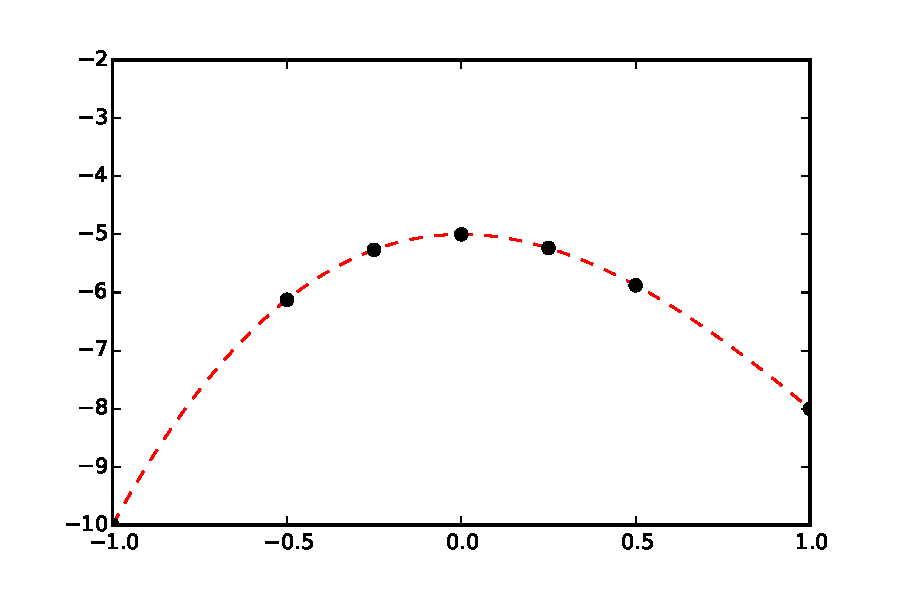
\includegraphics[width=10cm]{img/interpol1.pdf}
\caption{The black points represent known values of an otherwise unknown function. The dashed line represents an approximation to the unknown function in terms of a polyonmial of order $n-1$.}
\label{fig:interpol1}
\end{figure}

\begin{figure}[H]
\centering
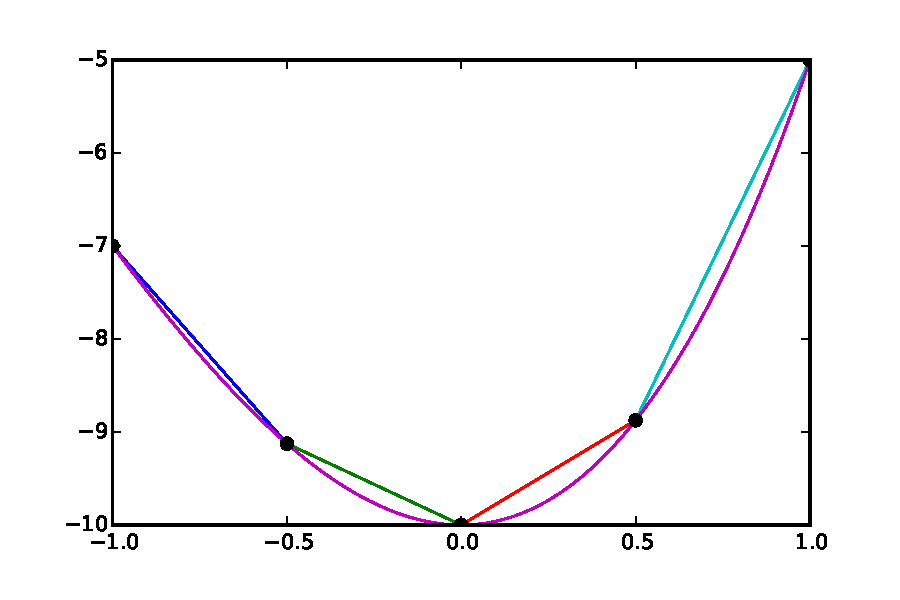
\includegraphics[width=10cm]{img/interpol2.pdf}
\caption{Interpolation takes place inside each sub-interval producing a piecewise interpolation approximation to the unknown function}
\label{fig:interpol2}
\end{figure}

\section{One-dimensional scalar functions}
\subsection{Lagrange interpolation theorem}
Given a set of n-points $\{ (x^1, y^1),\cdots,(x^n, y^n)\}$ where $y^n \equiv f({x^n})$ then: ``there exists a unique polynomial $p(x)$ of order at most $(n-1)$ such $p(x^I) = f(x^I)$ for $I=1,2,\cdots,n$". The polynomial is given by;

\begin{equation}\label{eq:inter_expl}
p(x) = {L^1}(x)f({x^1}) + {L^2}(x)f({x^2}) +  \ldots  + {L^n}(x)f({x^n})
\end{equation}

and the term ${L^I}(x)$ is computed as;

\begin{equation}\label{eq:coef}
  L^I(x) = \prod_{\substack{J = 1\\ I \ne J}}^n \frac{(x - x^J)}{(x^I - x^J)}.
\end{equation}

The approximate function $p(x)$ of order $n-1$ is termed {\bf the interpolating polynomial} such


\[f(x)\simeq p(x)\]


while each one of the terms ${L^I}(x)$, also of order $n-1$, are termed {\bf the interpolation functions}. In the context of the finite element method these are also called {\bf shape functions}.

The use of index notation, and particularly the summation convention, can be extended to represent the linear superposition of functions given by \cref{eq:inter_expl}. We use capital super-scripts to denote interpolation in such a way that a capital superscript denotes a data point in the interpolation scheme. Accordingly \cref{eq:inter_expl} can be equivalently written like:


\begin{equation}\label{eq:pol}
  p(x^I) = L^I(x) f(x^I)  
\end{equation}

where the fact that $I=1,2,...,n$ is implicit in the notation.

Recall that the interpolating polynomial $p(x)$ is just an approximation to the actual function $f(x)$. However, the approximation should at least be such that $p(x^I) = f(x^I)$ at the $n$ nodal points. To satisfy this condition the interpolation polynomials must be such that:

\[L^I(x^J) = \delta^{IJ}\]

and where ${\delta ^{IJ}}$ is the delta function extended to the interpolation polynomials.

\begin{tcolorbox}
The approximate function $p(x)$ resulting from the interpolation process is called the {\bf interpolating polynomial} while the Lagrange polynomials $L^I(x)$ are called interpolation functions. In the language of the finite element methods these are simply called {\bf shape functions}. 
\end{tcolorbox}


\begin{tcolorbox}
\paragraph*{A note regarding superscripts in indicial notation:} In this Class Notes superscripts associated to symbols like in the expression $x^4$ are frequently used to describe a variable associated to a nodal point: for instance, in this context the expression $x^4$ represents the $x$-coordinate of nodal point $4$. However, in some other cases this same expression might appear, for example, in the definition of a function like in $f(x) = {x^4} + 4{x^3}$. In both cases the specific meaning should be clear by the context in which it appears.

Python function {\bf LagrangPoly()} in NB-1 generates Lagrange interpolation polynomials of different order and over a varying range.
\end{tcolorbox}

\paragraph*{Example: Interpolation of a function using 3 data points}

Use a Lagrange interpolation scheme to find an interpolating polynomial that approximates the function 

\[ f(x) = {x^3} + 4{x^2} - 10 \]

at the sampling (or also nodal) points ${x^1} =  - 1.0$, ${x^2} =  + 1.0$ and ${x^3} = 0.0$ over the interval $[-1,1]$ together with its first order derivative at $x = 0.7$.  Assume that the values of the first derivative at the nodal points are unknown. 

\Cref{ejemplo2} contains the exact values for the function

\begin{center}
\begin{tabular}{ll}
  \hline
  $x$ & $f(x)$ \\
  \hline 
  $-1.0$  & $-7.000$  \\
  $ 0.00$  & $-10.00$  \\
  $ 1.00$  & $-5.000$  \\
  \hline
\end{tabular}
\captionof{table}{Known values of the function $f(x) = {x^3} + 4{x^2} - 10$ over the interval $[-1,1]$}
\label{ejemplo2}
\end{center}

The formulation of the interpolation scheme consists in finding the interpolation polynomials $L^I(x)$ and the interpolating function $p(x)$. From \cref{eq:coef} the interpolation functions, shown in \cref{fig:pols}, are:
\begin{align*}
L^1(x) = \frac{(x - x^2)(x - x^3)}{(x^1 - x^2)(x^1-x^3)} & \equiv  - \frac{1}{2}(1 -  x)x\\
L^2(x) = \frac{(x - x^1)(x - x^3)}{(x^2 - x^1)(x^2 - x^3)} & \equiv +   \frac{1}{2}(1 + x)x\\
L^3(x) = \frac{(x - x^1)(x - x^2)}{(x^3 - x^1)(x^3 - x^2)} & \equiv + (1 - x^2).
\end{align*}

\begin{figure}[H]
  \centering
  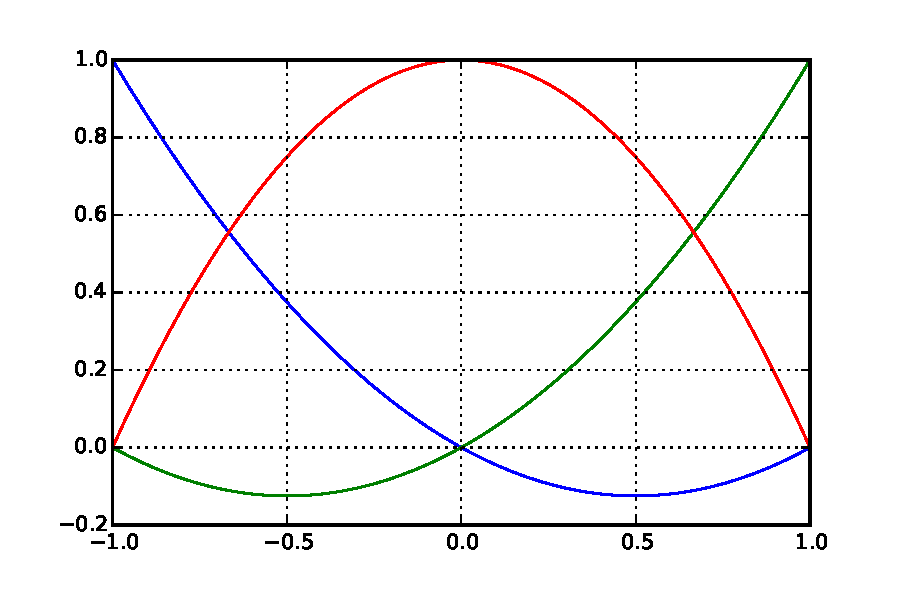
\includegraphics[width=10cm]{func1.pdf}
  \caption{(top) Interpolation polynomials $L^1(x)$, $L^2(x)$ and $L^3(x)$ as per \cref{eq:coef} computed for a second order scheme with 3 nodal points.}
  \label{fig:pols}
\end{figure}

The interpolating polynomial approximating the function is obtained using \cref{eq:pol} which in this case is given by


\[p(x) = 10{x^2} + \frac{7}{2}(1 - x)x - \frac{5}{2}(1 + x)x - 10.\]

The approximate and actual function are compared in \cref{fig:functions}. Clearly $p(x)$, being a second order function differs with $f(x)$, which is a third order function. However, as stated in the interpolation theorem both functions coincide at the nodal points where the known values of the function are available.


\begin{figure}[H]
  \centering
  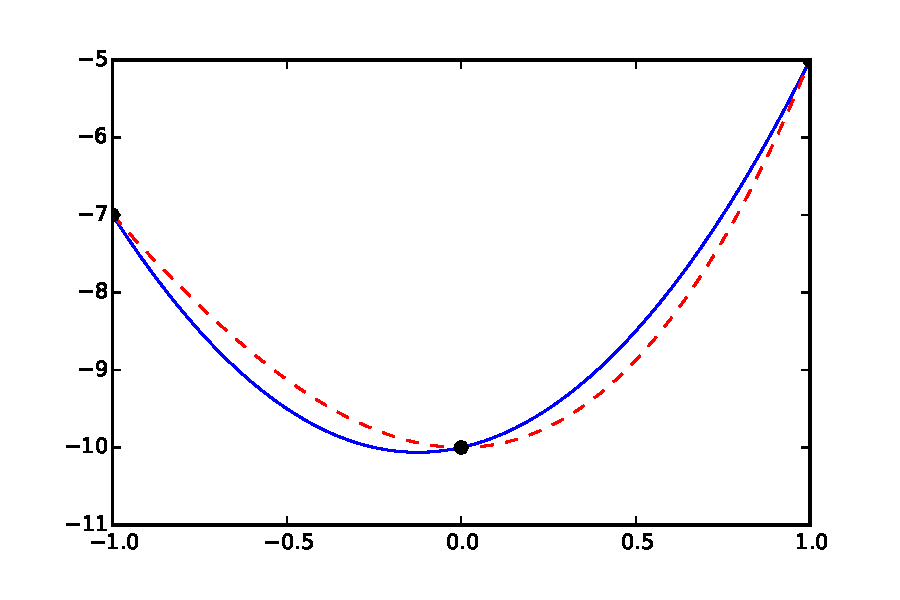
\includegraphics[width=10cm]{func2.pdf}
  \caption{Resulting interpolating function $p(x)$ as per \cref{eq:pol} compared with the exact function $f(x) = {x^3} + 4{x^2} - 10$. The Python code used for the interpolation is available in NB-1}
  \label{fig:functions}
\end{figure}


In finding an approximations to the first derivative recall that at the nodal points the values of these first derivatives are unknown. Thus the only available choice is to operate directly on $p(x)$ and use it to approximate also the first derivative like:


\begin{equation}\label{eq:der}
  \frac{ dp(x)}{dx} = \frac{dL^1(x)}{dx} f^1 + \frac{dL^2(x)}{dx}(x) f^2 + \frac{dL^3(x)}{dx} f^3
\end{equation}

It is evident that the approximation takes the form of a lineal superposition of products between interpolation functions (which in this case are derivatives of the $L^I$) and known values of the function. The first derivative obtained in this form differs from the actual derivative of $f(x)$ since this approach uses the values of $f$ and not those of $\frac{{df(x)}}{{dx}}$ and $\frac{dL^I(x)}{dx}$ instead of $L^I$ and these functions do not satisfy the condition $\frac{dL^I(x^J)}{dx} = \delta ^{IJ}$.


\begin{figure}[H]
  \centering
  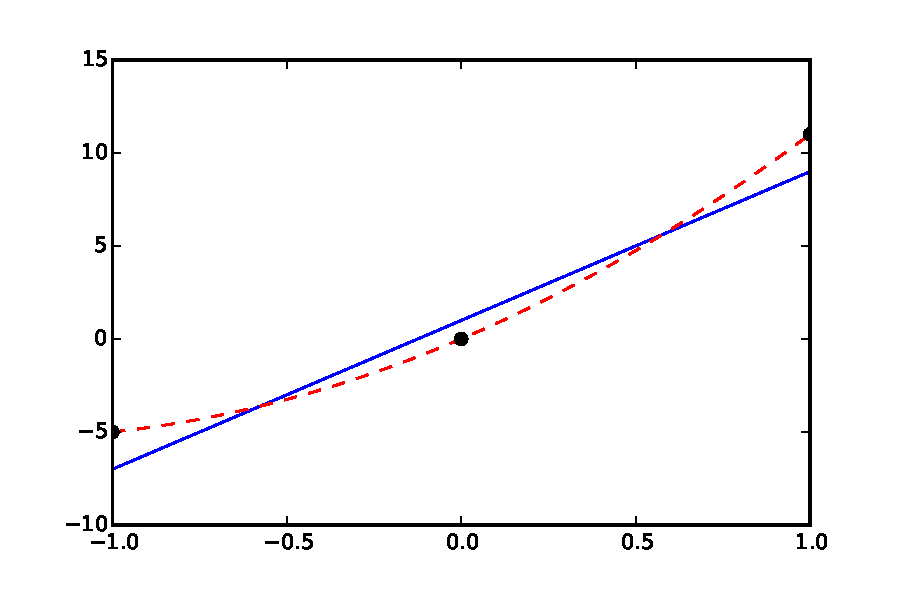
\includegraphics[width=10cm]{deriv.pdf}
  \caption{Comparison between the first order derivative of $p(x)$ with the closed-form result of $\frac{{df(x)}}{{dx}}$}
  \label{fig:deriv}
\end{figure}


\Cref{fig:first der 1} shows the approximation to $f'(x)$ when $p(x)$ is computed using 4th-order polynomials.

\begin{figure}[H]
  \centering
  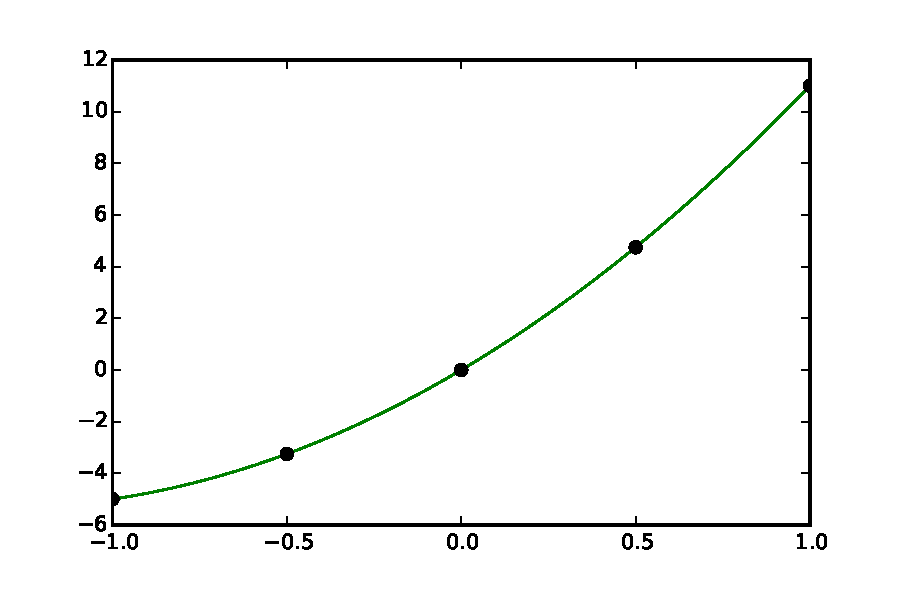
\includegraphics[width=10cm]{firstder.pdf}
  \caption{Comparison between the first order derivative of $p(x)$ computed using 4th-order polynomials with the closed-form result of $\frac{{df(x)}}{{dx}}$}
  \label{fig:first der 1}
\end{figure}

To identify the variation in the solution with different interpolation schemes \cref{fig:several interpol} compares the exact and interpolated solution for polynomials of order 1, 2 and 4 respectively. The left column displays the interpolation polynomials ${{L^I}(x)}$.

\begin{figure}[H]
\centering
	\begin{subfigure}[b]{0.450\textwidth}\qquad
		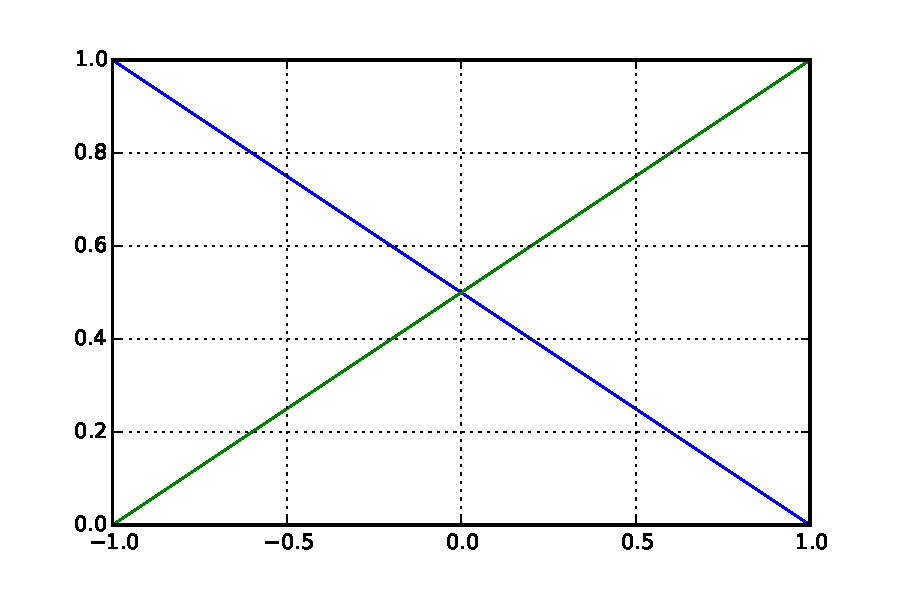
\includegraphics[width=\textwidth]{lineal.pdf}
		\caption{First order. }
	\end{subfigure}\,
%
	\begin{subfigure}[b]{0.450\textwidth}\qquad
		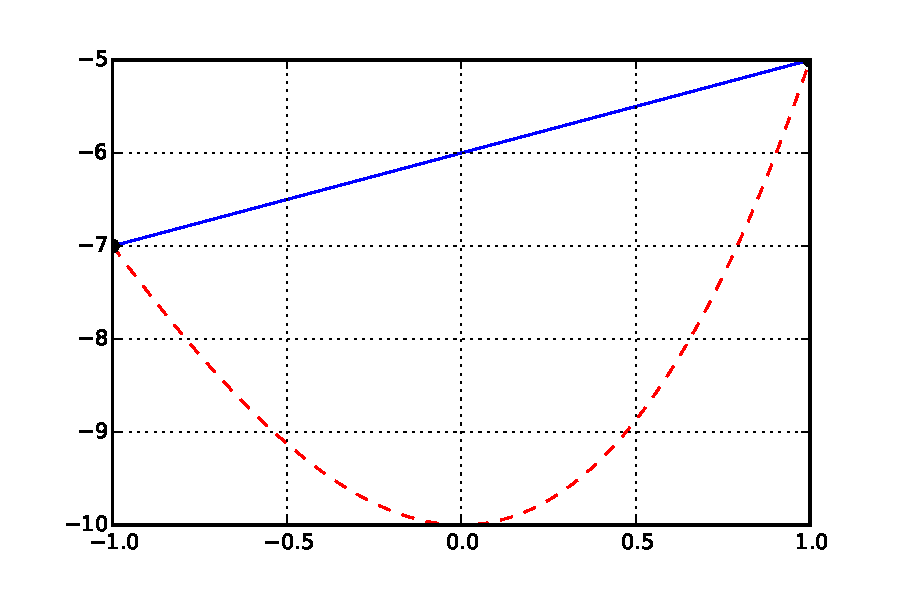
\includegraphics[width=\textwidth]{interlin.pdf}
		\caption{Actual and interpolated function.}
	\end{subfigure}\\
%
\centering
	\begin{subfigure}[b]{0.450\textwidth}\qquad
		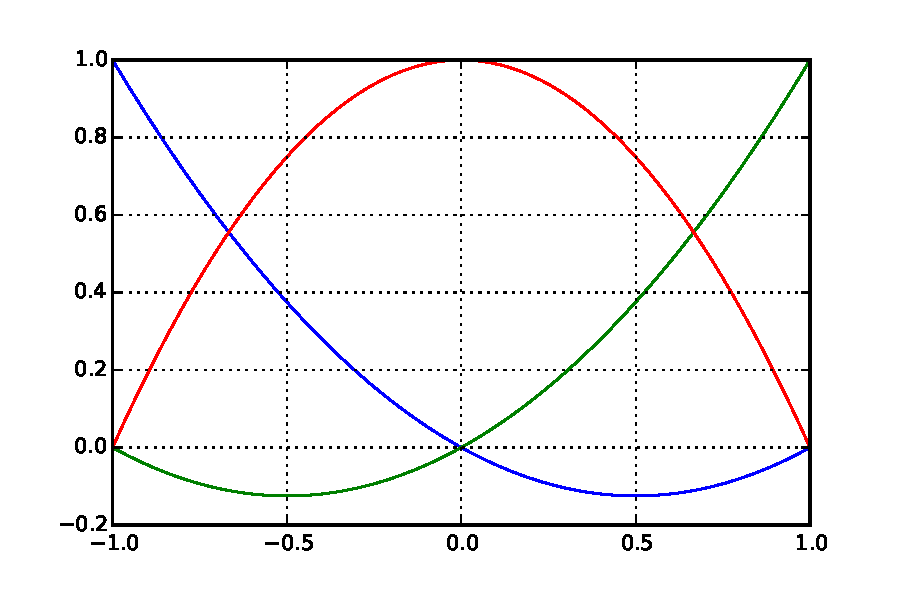
\includegraphics[width=\textwidth]{quadra.pdf}
		\caption{Second order.}
	\end{subfigure}\,
%
	\begin{subfigure}[b]{0.450\textwidth}\qquad
		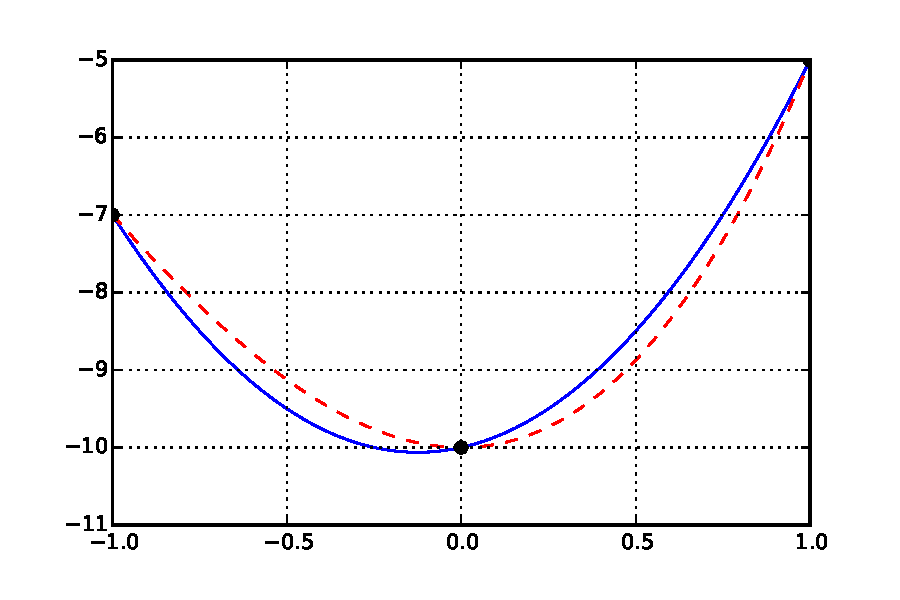
\includegraphics[width=\textwidth]{interqua.pdf}
		\caption{Actual and interpolated function.}
	\end{subfigure}\\
%
\centering
	\begin{subfigure}[b]{0.450\textwidth}\qquad
		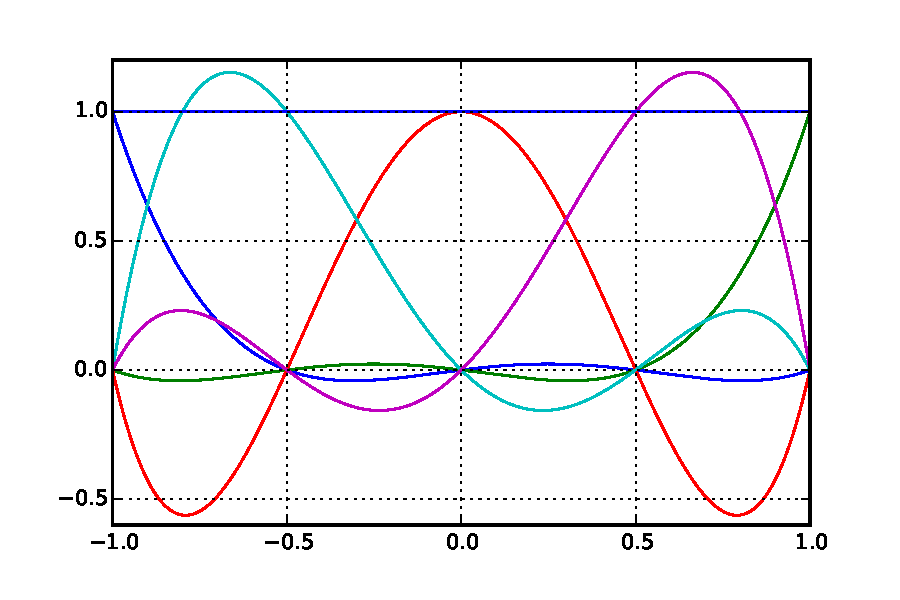
\includegraphics[width=\textwidth]{third.pdf}
		\caption{Fourth order.}
	\end{subfigure}\,
%
	\begin{subfigure}[b]{0.450\textwidth}\qquad
		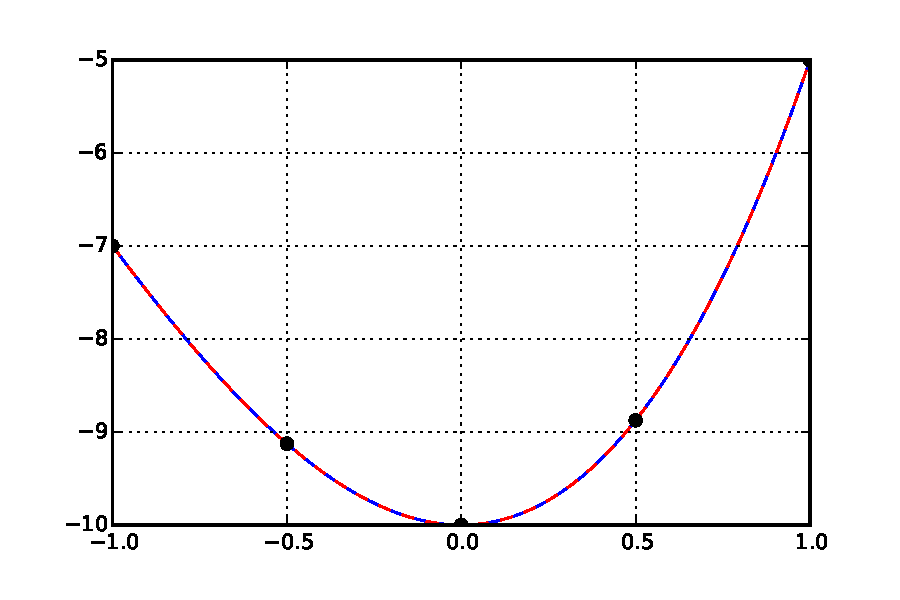
\includegraphics[width=\textwidth]{intertri.pdf}
		\caption{Actual and interpolated function.}
	\end{subfigure}
\caption{Interpolation of the function $f(x) = {x^3} + 4{x^2} - 10$ using Lagrange polynomials of increasing order.}
\label{fig:several interpol}
\end{figure}

\subsection{Local interpolation using a piece-wise continuous function}
An alternative to the non-uniform nodal distribution approach used in the previous section to improve the interpolation scheme is based on splitting the solution interval $[x_1, x_n]$ in smaller sub-domains where the interpolation is performed locally. For instance \cref{subdo} shows such a partition for the interval $[-1.0, 1.0]$ where each sub-domain is conformed by a pair of consecutive nodes. The table shows values of the function $f(x) = {x^3} + 4{x^2} - 10$ at the edges of the sub-domains. In this particular case, considering each sub-domain to be conformed by a pair of points, the lineal interpolation scheme reduces to finding the straight line (first order polynomial) that passes along the pair of nodes. Higher order local schemes are possible if additional points are added to the sub-domains.

\begin{center}
\begin{tabular}{ccc}
  \hline
  Subdomain & Range & Values for $f(x)$ \\
  \hline 
   1  & $[-1.0, -0.5]$ & $[-7.000, -9.125]$  \\
   2  & $[-0.5,  0.00]$ & $[-9.125, -10.00]$  \\
   3  & $[+0.0,  +0.5]$ & $[-10.00, -8.875]$   \\
   4  & $[+0.5, +1.0]$ & $[-8.875, -5.000]$   \\
  \hline
\end{tabular}
\captionof{table}{Partition of the interval $[-1.0, 1.0]$ into subdomains}
\label{subdo}
\end{center}

\begin{tcolorbox}

Using piecewise interpolation over constant size intervals implies also the use of constant polynomials. In the finite element method each sub-domain is mapped into a constant size interval facilitating systematization of the interpolation process.
Notebook 2 in the REPO shows the Python implementation of piecewise interpolation.

\end{tcolorbox}


\begin{figure}[H]
  \centering
  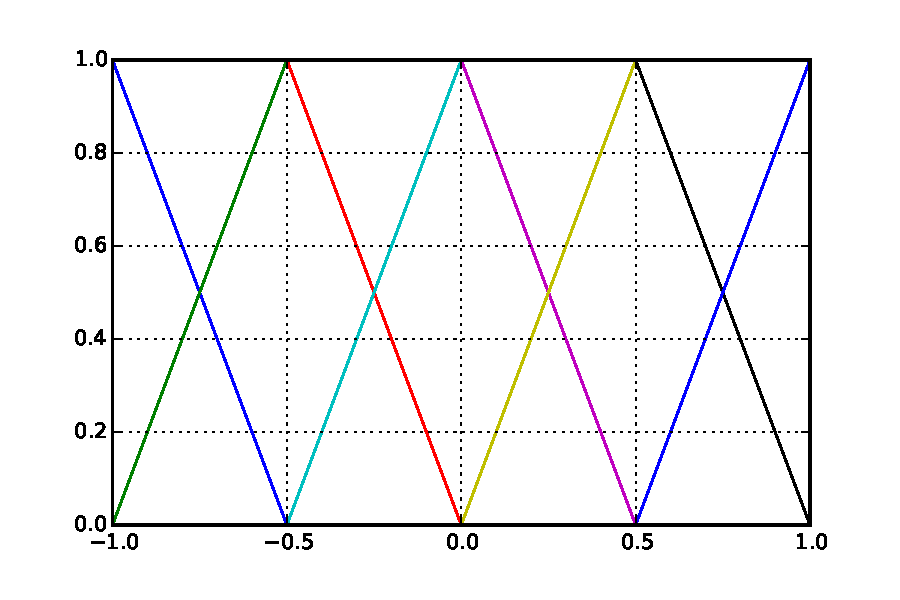
\includegraphics[width=10cm]{localone.pdf}
  \caption{Local interpolating polynomials.}
  \label{fig:loc-pols}
\end{figure}

This approach results in an interpolating polynomial as shown in \cref{fig:fully local 1} and where the approximated function is piece-wise continuous. As a result the local based technique the first derivative of the function is now discontinuous at the boundaries of the subdomains. However this local schema is advantageous since the local polynomials are unique and the scheme can be used for an arbitrary number of nodal points facilitating computer implementation.


\begin{figure}[H]
\centering
	\begin{subfigure}[b]{0.45\textwidth}\qquad
		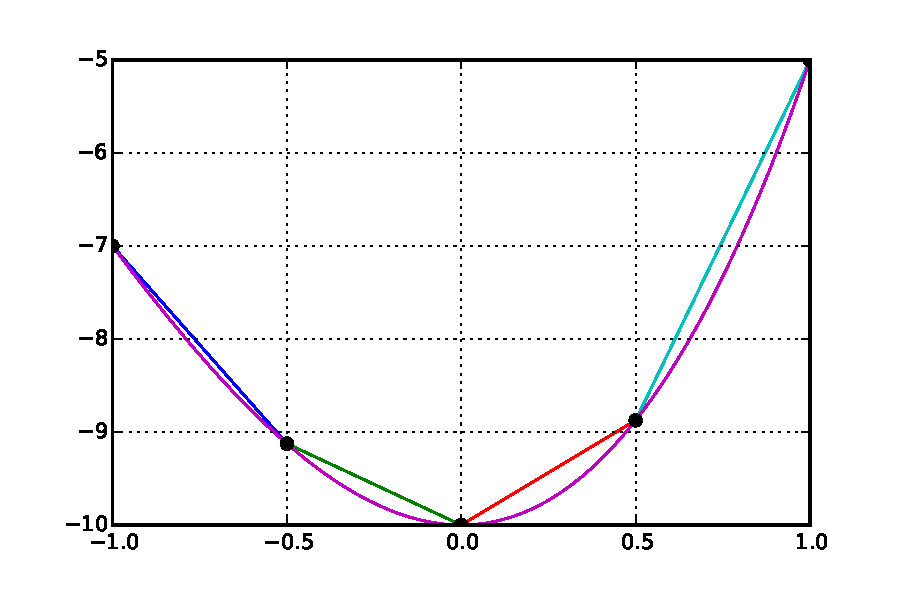
\includegraphics[width=\textwidth]{localfun.pdf}
		\caption{Approximation to the function using first order interpolation polynomials.}
	\end{subfigure}\,
%
	\begin{subfigure}[b]{0.45\textwidth}\qquad
		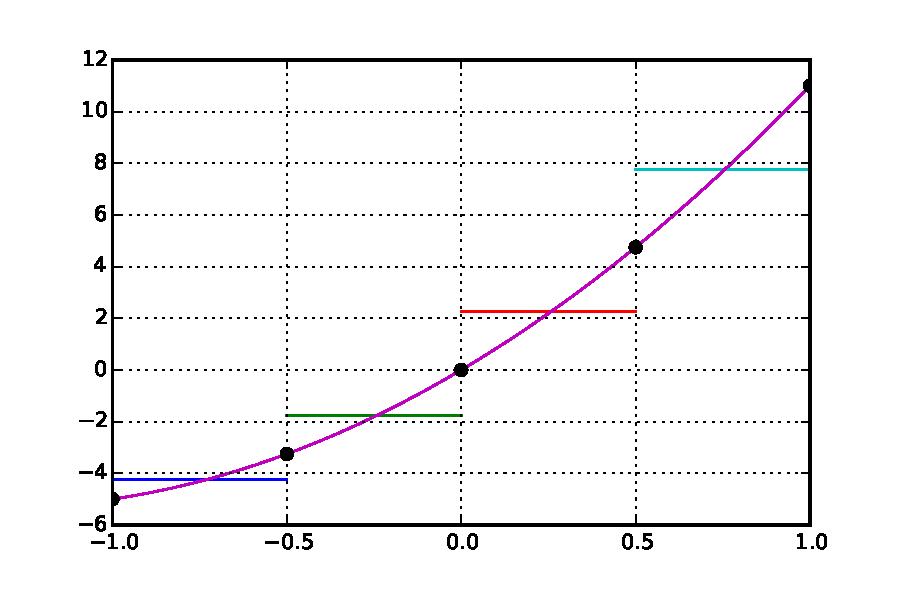
\includegraphics[width=\textwidth]{localfirst.pdf}
		\caption{Variation of the first order derivative.}
	\end{subfigure}\\

\caption{Locally based interpolation scheme for the function $f(x) = {x^3} + 4{x^2} - 10$.}
\label{fig:fully local 1}
\end{figure}



\subsection{Distribution of the sampling (or nodal) points}
The simple problems considered so far have used a small number of sample points and a constant separation distance. This approach worked nicely considering the smooth functions involved. However if the function to be interpolated exhibits strong gradients, as might be the case in problems of wave propagation, the approximation with a small number of data points is very likely insufficient. The natural solution seems to be the addition of data points and thus an increase in the order of the interpolating polynomial. Unfortunately, as we will show here this approach does not always works in the desired direction.


Consider the function:

\[f(x) = \frac{1}{{1 + 25{x^2}}}\]

shown in \cref{fig:rungelag}.

\begin{figure}[H]
\centering
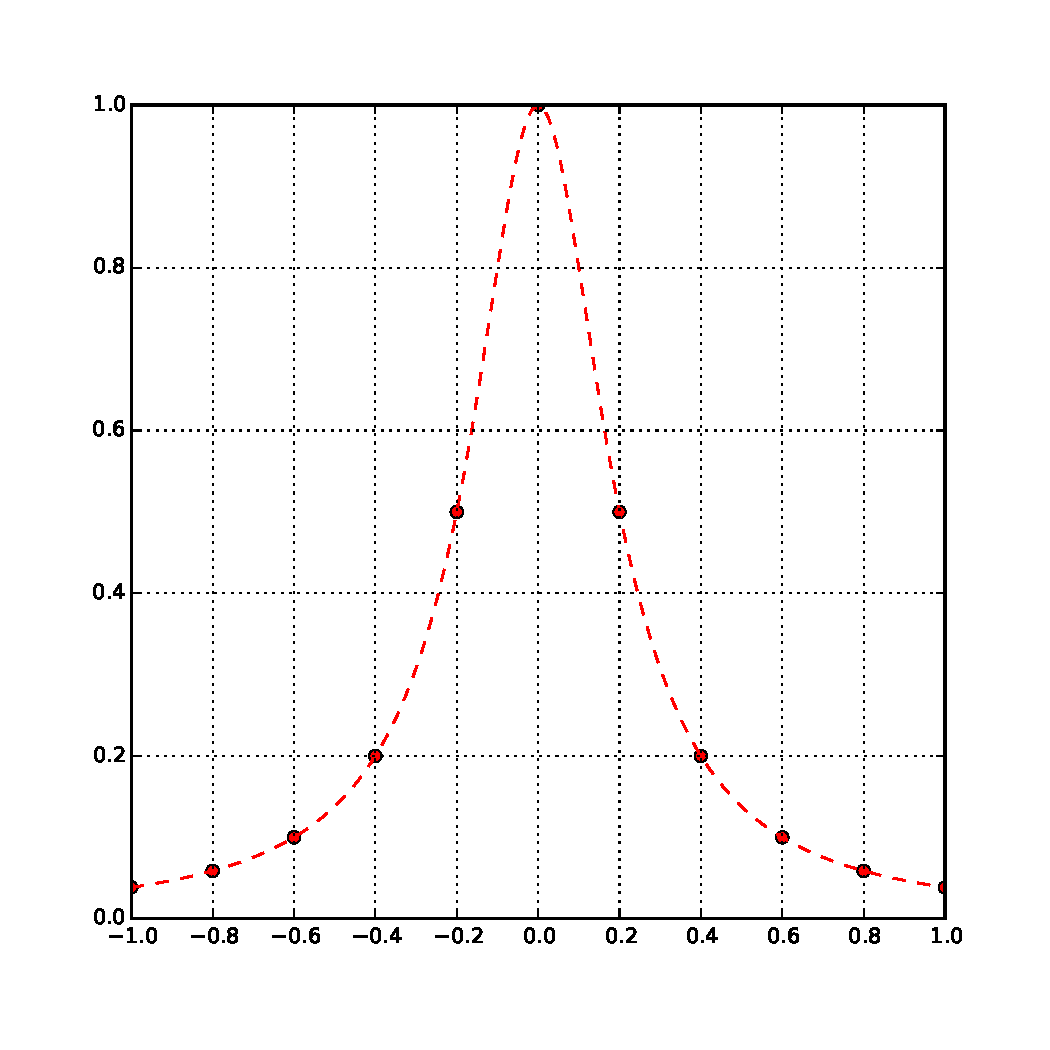
\includegraphics[width=8cm]{runge.pdf}
\caption{Runge function $f(x) = \frac{1}{1 + 25{x^2}}$.}
\label{fig:rungelag}
\end{figure}

This function shows a strong spatial variation requiring an interpolating polynomial of larger order and as a result a larger number of nodal points. The 11 black dots shown in the figure represent nodal points equally spaced at $\Delta x = 0.2$ and where the function is assumed to be known. We wish to approximate this function using these 11 points and an order 10 interpolating Lagrange polynomial.



\Cref{fig:rungeequi} shows the 11 order-10 Lagrange interpolation polynomials for the equidistant nodal distribution and the resulting interpolating polynomial $p(x)$. Clearly the approximation is highly inaccurate, specially near the edges of the interval where it exhibits strong oscillations. This spurious result along the edges is introduced by the equidistant separation of the sampling points. The interpolation scheme can be improved using a non-uniform nodal spacing. The resulting alternative scheme is shown in  \cref{fig:rungechevy} where there is a large concentration of nodal points along the edges.

\begin{figure}[H]
\centering
	\begin{subfigure}[b]{0.50\textwidth}\qquad
		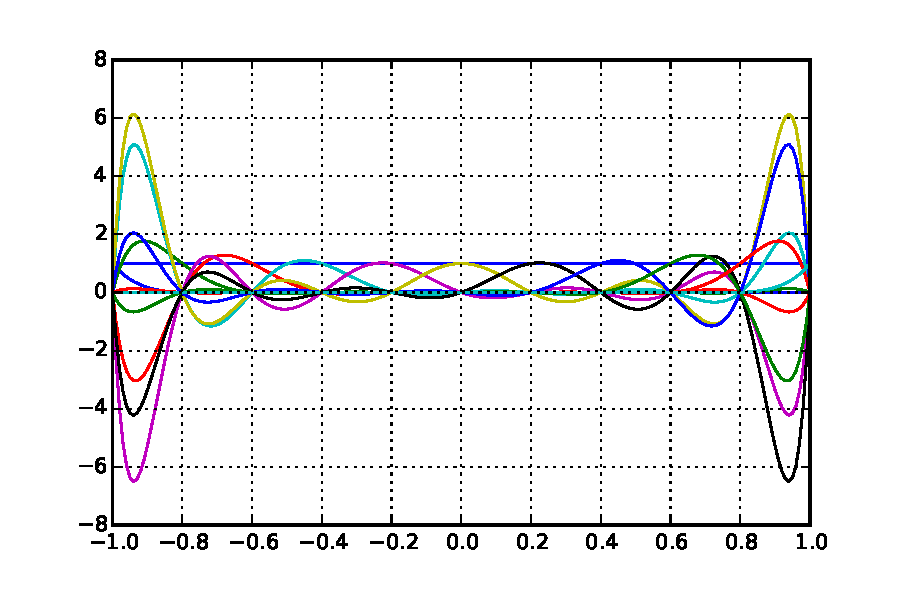
\includegraphics[width=\textwidth]{lag11.pdf}
		\caption{}
	\end{subfigure}\,
%
	\begin{subfigure}[b]{0.45\textwidth}\qquad
		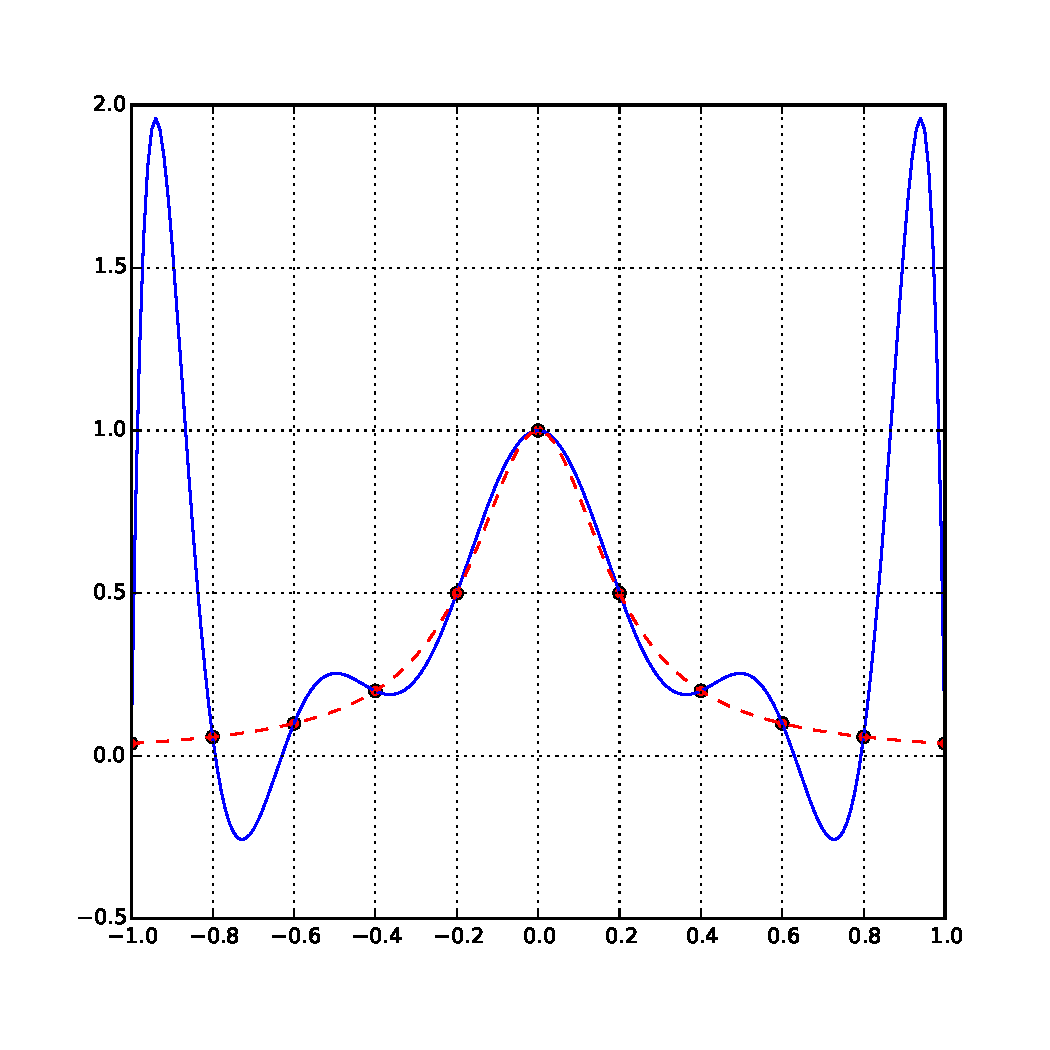
\includegraphics[width=\textwidth]{rungaprlag.pdf}
		\caption{}
	\end{subfigure}\\

\caption{(a) Lagrange interpolation polynomials of order 10 associated to the 11 sampling points for \cref{fig:rungelag}. (b) Interpolating polynomial to approximate the Runge function with the order-10 polynomials from part (a).}
\label{fig:rungeequi}
\end{figure}


\begin{figure}[H]
\centering
	\begin{subfigure}[b]{0.50\textwidth}\qquad
		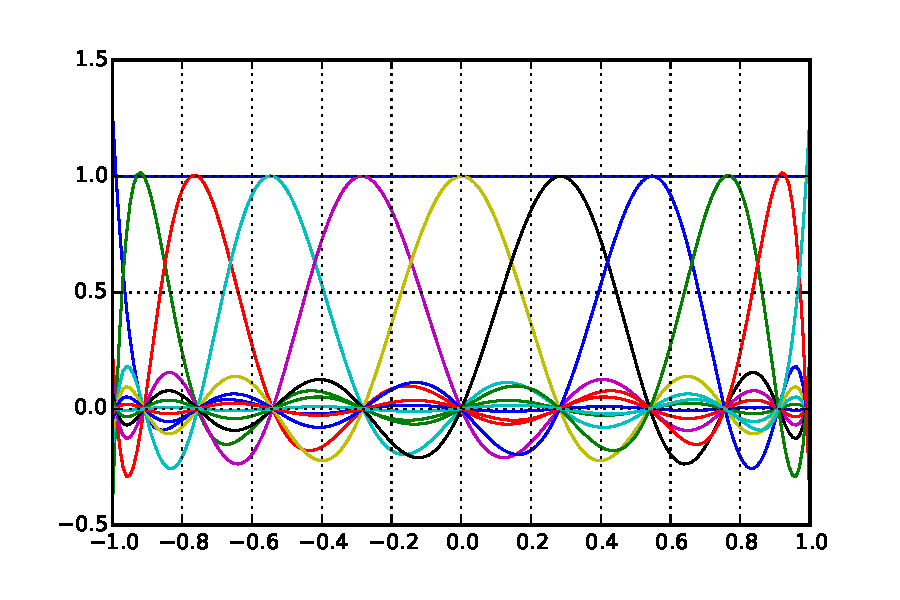
\includegraphics[width=\textwidth]{lagchv.pdf}
		\caption{}
	\end{subfigure}\,
%
	\begin{subfigure}[b]{0.45\textwidth}\qquad
		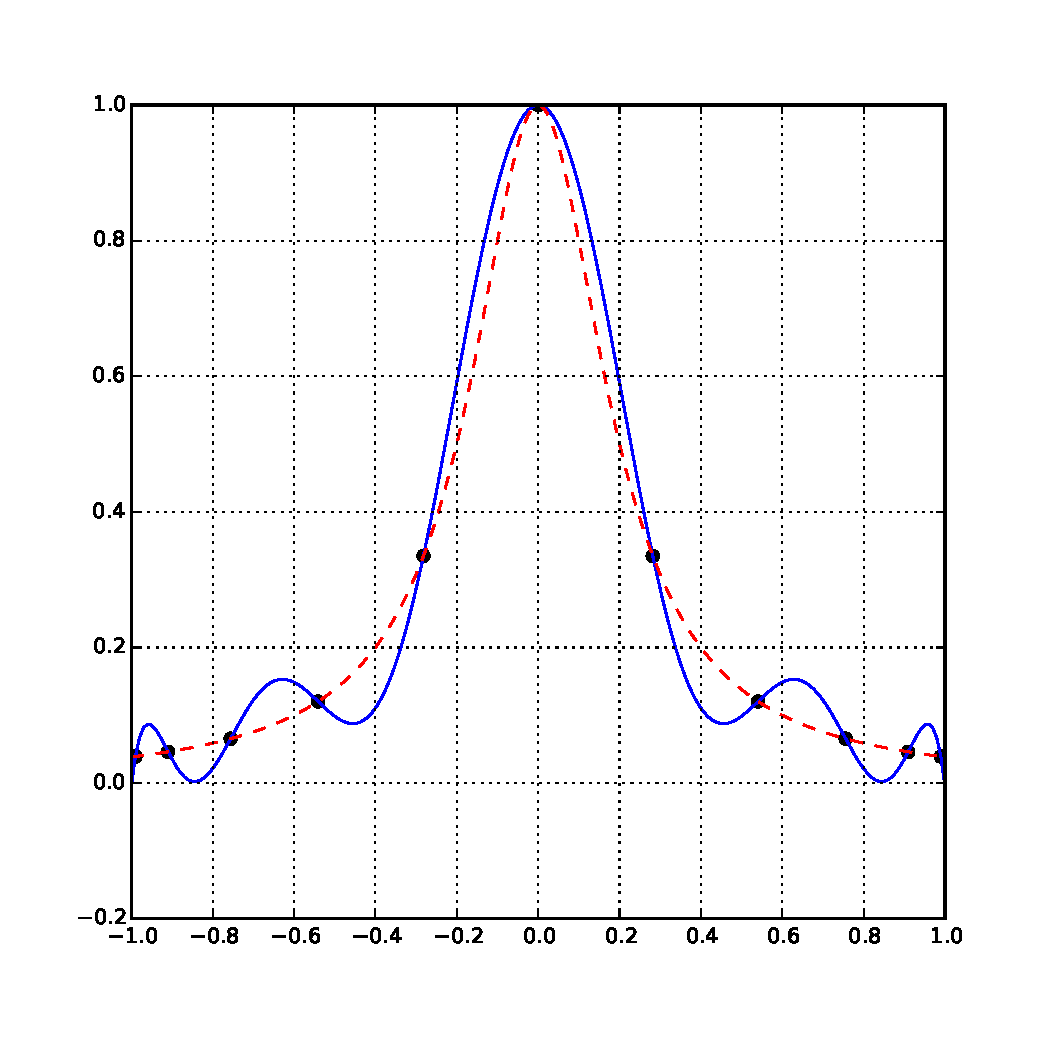
\includegraphics[width=\textwidth]{rungaprchv.pdf}
		\caption{}
	\end{subfigure}\\

\caption{(a) Order 10 Lagrange interpolation polynomials associated to non-equidistant sampling points. (b) Interpolating polynomial to approximate a Runge function built with the polynomials derived in part (a).}
\label{fig:rungechevy}
\end{figure}

To understand this numerical pathology, related with the distribution of the nodal points, consider the interpolation polynomials corresponding to the central point and to the edge point of the equidistant distribution (\cref{fig:rungeequi}) as shown in part(a) of \cref{fig:compara}. The green line corresponds to the polynomial associated to the central node, while the blue line is that of the edge nodal point. Clearly, the central-point polynomial introduces a strong variation along the edges of the sampling interval, while the edge-point polynomial exhibits a rather smooth variation. Similarly, part(b) in the same figure shows once again the central-point and the edge-point polynomials associated to non-uniform nodal distribution. It can be observed how in this last case both polynomials exhibit a smooth variation over the interval eliminating the strong oscillation towards the edges.

\begin{figure}[H]
\centering
	\begin{subfigure}[b]{0.45\textwidth}\qquad
		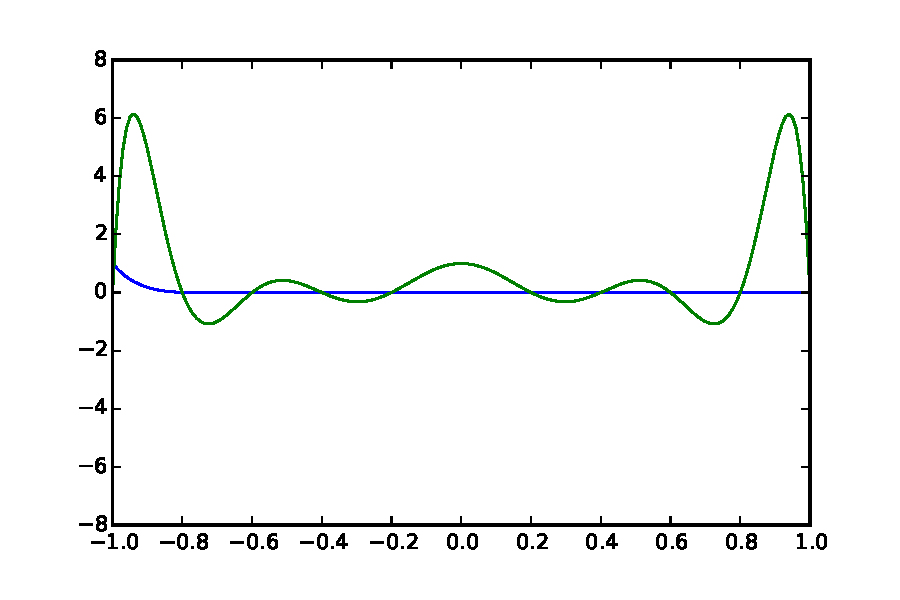
\includegraphics[width=\textwidth]{central.pdf}
		\caption{}
	\end{subfigure}\,
%
	\begin{subfigure}[b]{0.45\textwidth}\qquad
		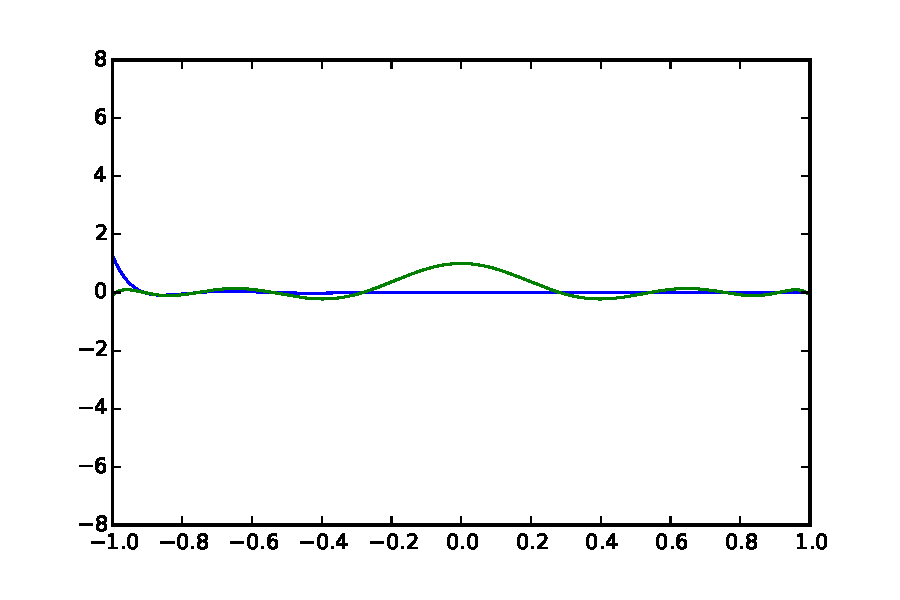
\includegraphics[width=\textwidth]{extremo.pdf}
		\caption{}
	\end{subfigure}\\

\caption{(a) Equidistant nodal points (b) Non-uniform nodal points.}
\label{fig:compara}
\end{figure}

\section{Extension to two-dimensional domains}
Assume we are now interested in conducting interpolation of a function over a spatial 2-dimensional domain where every point is specified by a position vector of the form $\overrightarrow x = x \hat{\imath} + y\hat{\jmath}$. We want to know, via interpolation, the value of a function $f(\overrightarrow x)$ at an arbitrary point $\overrightarrow x$ provided we know the set of n-pairs of the form $\{(\overrightarrow x ^1, f^1),\cdots,(\overrightarrow x ^n, f^n)\}$. The domain and the visualization of the function are shown in \cref{fig:element}.

\begin{figure}[H]
\centering
	\begin{subfigure}[b]{0.45\textwidth}\qquad
		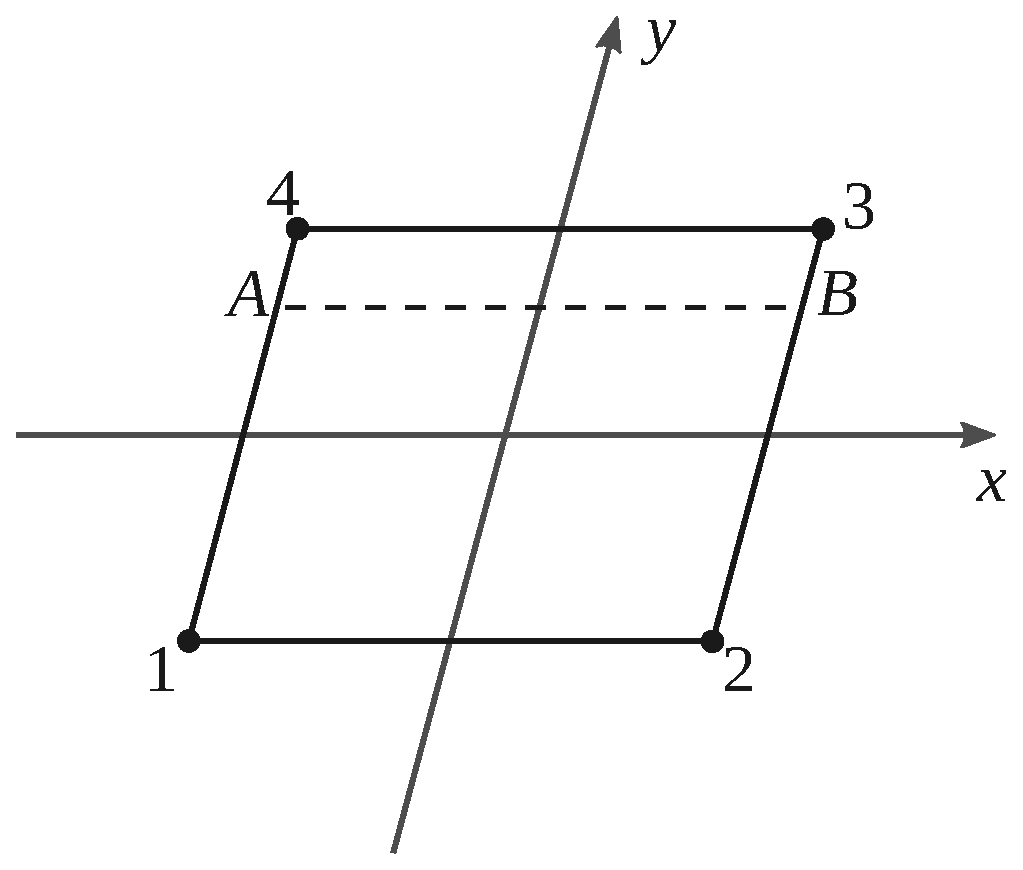
\includegraphics[width=\textwidth]{element.pdf}
		\caption{Square two-dimensional domain}
	\end{subfigure}\,
%
	\begin{subfigure}[b]{0.45\textwidth}\qquad
		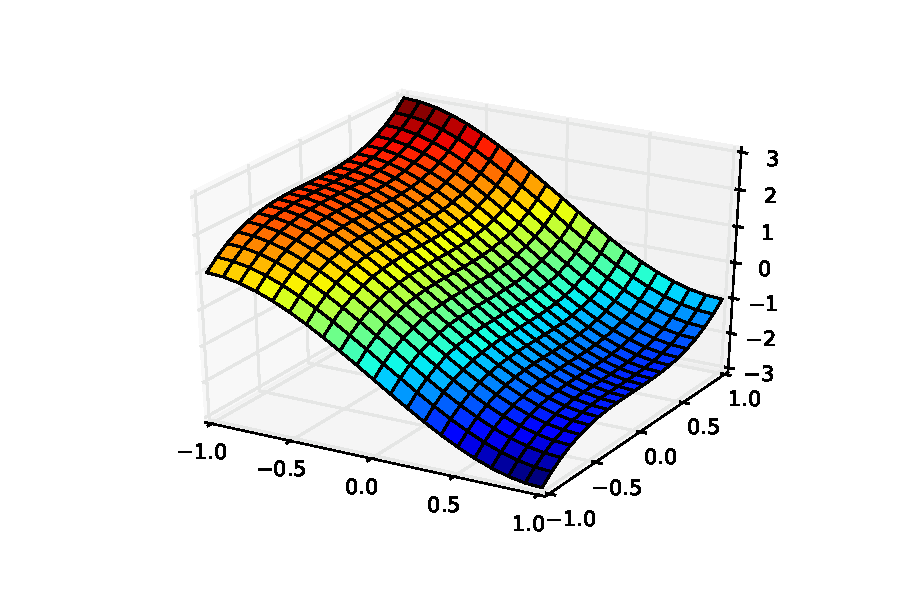
\includegraphics[width=\textwidth]{surface.pdf}
		\caption{Interpolated function $f(x,y)$.}
	\end{subfigure}\\

\caption{Function $f(x,y)$ over a square two-dimensional domain with nodal points labeled 1 , 2 , 3 , 4.}
\label{fig:element}
\end{figure}

Since now the function $f$ depends on the 2D space coordinates $(x , y)$ it is natural to expect that interpolation functions depend also on $(x , y)$. Using this condition on the function approximation we have:

\[f(x,y) = N^1(x,y)f^1 + N^2(x,y)f^2 + N^3(x,y)f^3 + N^4(x,y)f^4\]

where now $N^Q(x,y)$ is the 2D interpolation (or shape) function associated to the sampling point $Q$. Using indicial summation convention, we can write the interpolated function as:

\[f(x,y) = N^Q(x,y)f^Q\]

where now $Q = 1,...,N$.


The method to find the required 2D shape functions $N^Q(x,y)$ consists in the recursive (or iterated) application of the Lagrange one-dimensional scheme discussed previously in terms of interpolating polynomials $L^Q(\eta)$ and where now $\eta$ is a dummy variable that can assume the role of $x$ or $y$.

In the domain shown in  \cref{fig:element} assume that we wish to interpolate the value of the function along the 1-4 direction. Note that along this line x is constant and then the function depends only on $y$. Fixing $x = x^A$ it is possible to conduct 1-dimensional interpolation along the $y$ direction as shown in \cref{fig:onedimn}. In this case $\eta$ assumes the role of $y$ and we have:

\[f(x^A,y) = L^1(y)f^1 + L^4(y)f^4.\]

Since the interpolation scheme is taking place along the 1-4 direction in terms of the 2 nodal values $f^1$ and $f^4$, the functions $L^1$ and $L^4$ in this case are the first order Lagrange polynomials associated to the points 1 and 4 respectively, and obtained with the already known product formula given in \cref{eq:coef}.



Clearly, the above scheme provides the value of the function for an arbitrary point $A$ along the 1-4 line. Proceeding similarly along the 2-3 direction, that is setting $x = x^B$ and interpolating once again along the $y$ direction we have:
\[f(x^B,y) = L^2(y)f^2 + L^3(y)f^3.\]

\begin{figure}[H]
\centering
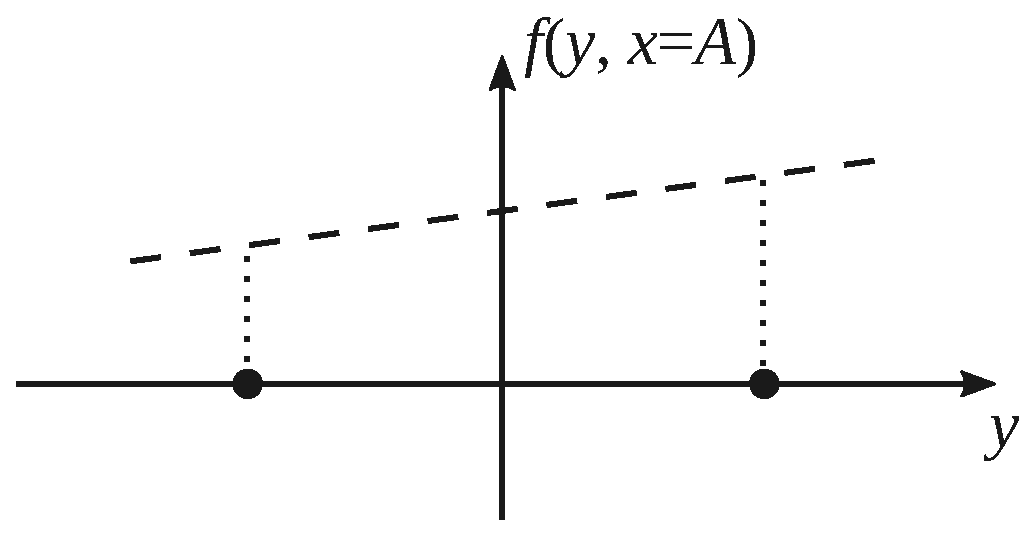
\includegraphics[width=10cm]{inter1D.pdf}
\caption{Interpolation along the $y$-direction}
\label{fig:onedimn}
\end{figure}



So far, we have captured only the dependence on $y$ since $x$ was assumed constant as indicated by $f(x^A,y)$ and $f(x^B,y)$. The dependence on $x$ is now captured proceeding similarly along the arbitrary line $A-B$ using the functions $f(x^A,y)$ and $f(x^B,y)$ respectively as follows;

\[f(x,y) = L^A(x) f(x^A,y) + L^B(x)f(x^B,y)\]

which after substituting with the found expressions for $f(x^A,y)$ and $f(x^B,y)$ becomes

\begin{align*}
  &f(x,y) = L^A(x)\{L^1(y)f^1 + L^4(y)f^4\} + L^B(x)\{L^2(y)f^2 + L^3(y)f^3\}\\
  &f(x,y) = L^A(x)L^1(y)f^1 + L^A(x)L^4(y)f^4 + L^B(x)L^2(y)f^2 + L^B(x)L^3(y)f^3 \enspace .
\end{align*}

Note that strictly speaking there are only 2 interpolation functions of the form $L^Q(\eta)$ since one-dimensional interpolation is taking place. Thus the interpolating polynomials satisfy the following equivalences:

where
\begin{align*}
L^A(x) & \equiv L^1(x)\\
L^B(x) & \equiv L^2(x)\\
L^1(y) & \equiv L^1(y)\\
L^2(y) & \equiv L^1(y)\\
L^3(y) & \equiv L^2(y)\\
L^4(y) & \equiv L^2(x) \enspace .
\end{align*}

The resulting two-variable shape functions $N^Q(x,y)$ follow from the product of one-dimensional interpolation functions like:

\begin{align*}
N^1(x,y) & = L^1(x)L^1(y)\\
N^2(x,y) & = L^2(x)L^1(y)\\
N^3(x,y) & = L^2(x)L^2(y)\\
N^4(x,y) & = L^1(x)L^2(y) \enspace .
\end{align*}

In the actual computer implementation of the discussed interpolation scheme it is desirable to have the actual functions embedded into the code instead of having the computer finding the corresponding Lagrange polynomials each time the size of the square domain changes. In practice, the functions $N^Q(x,y)$ are coded for a canonic square of general side $h$. This resulting canonic domain can be referred as a finite element.

\paragraph*{A 2D finite element}
From the geometric point of view a {\bf finite element} is a canonical interpolation domain together with a set of shape functions and its derivatives. \Cref{fig:four-nodes-interp} shows the shape functions for a so-called bi-linear element of side $h = 1.0$. The element is called bi-linear as linear (or first order) interpolation is used along the $x$ and $y$ directions. Elements of higher order result after adding nodal points and the required corrections to the 2D-shape functions $N^Q(x,y)$.

%The shape functions for a 9-noded element are displayed in \cref{fig:nine-nodes-interp}.

\begin{figure}[H]
\centering
	\begin{subfigure}[b]{0.45\textwidth}\qquad
		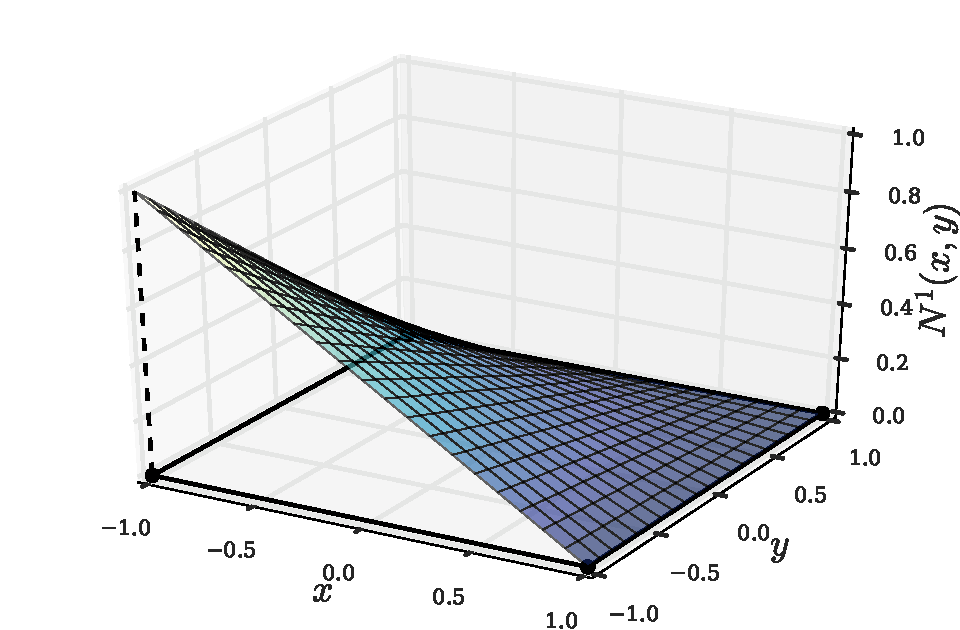
\includegraphics[width=\textwidth]{shape_func-4-nodes-1.pdf}
		\caption{Shape function ${N^1(x,y)=\frac{1}{4}(1-x)(1-y)}$. }
	\end{subfigure}\,
%
	\begin{subfigure}[b]{0.45\textwidth}\qquad
		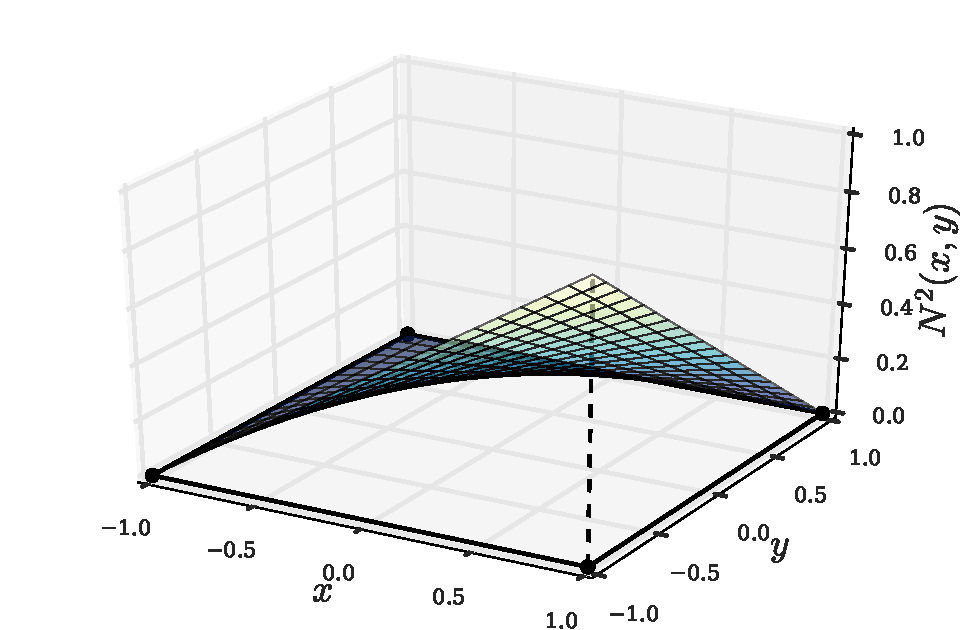
\includegraphics[width=\textwidth]{shape_func-4-nodes-2.pdf}
		\caption{Shape function ${N^2(x,y)=\frac{1}{4}(1+x)(1-y)}$.}
	\end{subfigure}\\
%
	\begin{subfigure}[b]{0.45\textwidth}\qquad
		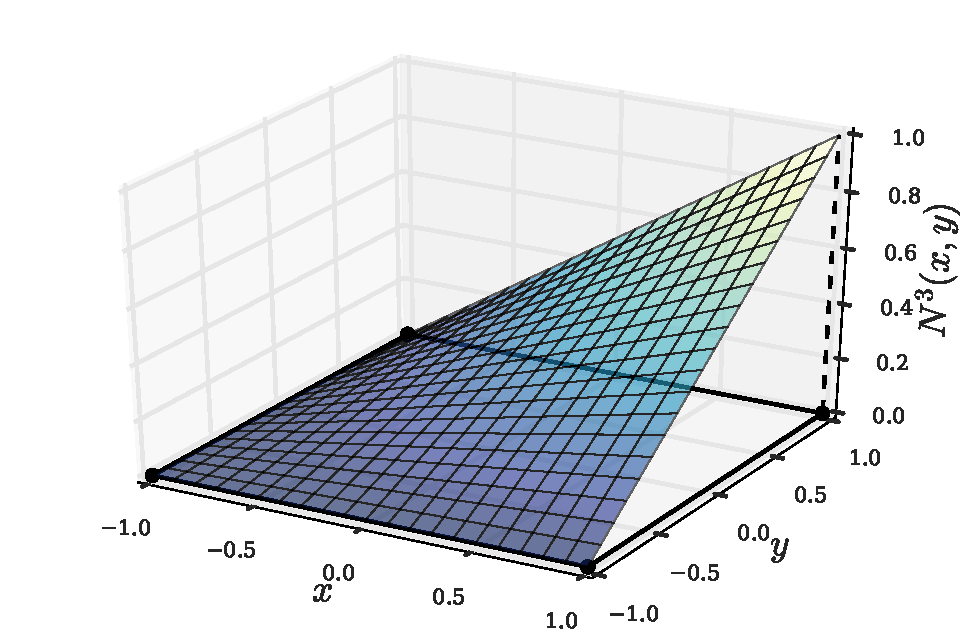
\includegraphics[width=\textwidth]{shape_func-4-nodes-3.pdf}
		\caption{Shape function ${N^3(x,y)=\frac{1}{4}(1+x)(1+y)}$.}
	\end{subfigure}\,
%
	\begin{subfigure}[b]{0.45\textwidth}\qquad
		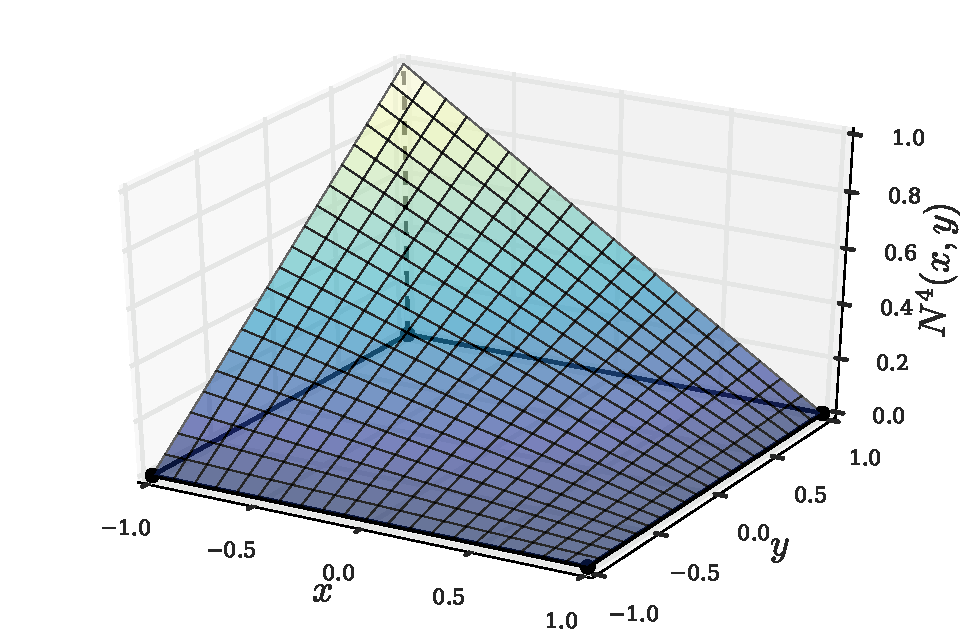
\includegraphics[width=\textwidth]{shape_func-4-nodes-4.pdf}
		\caption{Shape function ${N^4(x,y)=\frac{1}{4}(1-x)(1+y)}$.}
	\end{subfigure}
\caption{Shape functions for a 4-nodes element.}
\label{fig:four-nodes-interp}
\end{figure}

\begin{tcolorbox}

See Notebooks 3 and 4 for an easy to follow Python implementation of interpolation resembling the finite element method.

\end{tcolorbox}



%\begin{figure}[H]
%\centering
%	\begin{subfigure}[b]{0.45\textwidth}\qquad
%		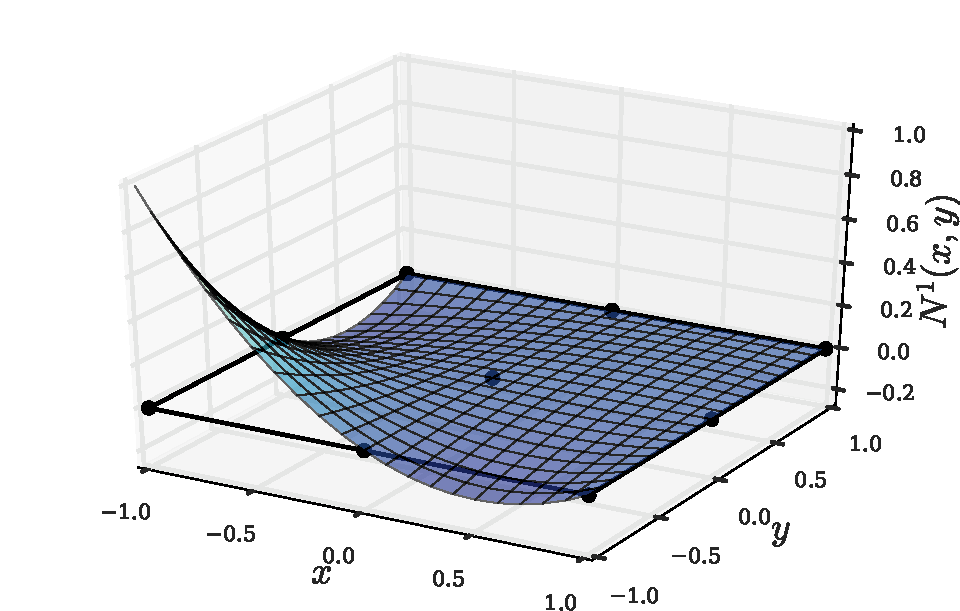
\includegraphics[width=\textwidth]{shape_func-9-nodes-1.pdf}
%		\caption{Shape function $N^1(x,y)$. }
%	\end{subfigure}\,
%%
%	\begin{subfigure}[b]{0.45\textwidth}\qquad
%		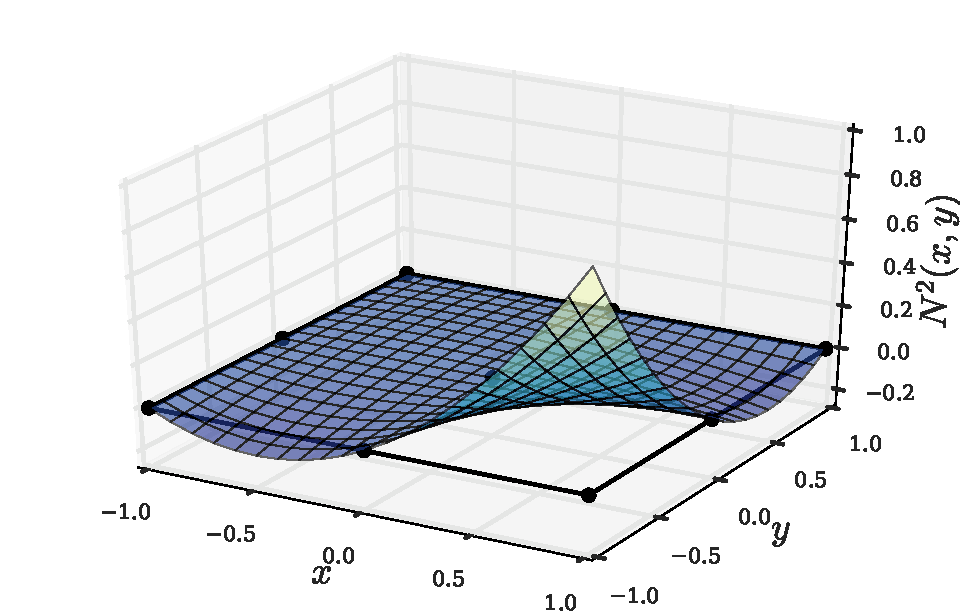
\includegraphics[width=\textwidth]{shape_func-9-nodes-2.pdf}
%		\caption{Shape function $N^2(x,y)$.}
%	\end{subfigure}\\
%%
%	\begin{subfigure}[b]{0.45\textwidth}\qquad
%		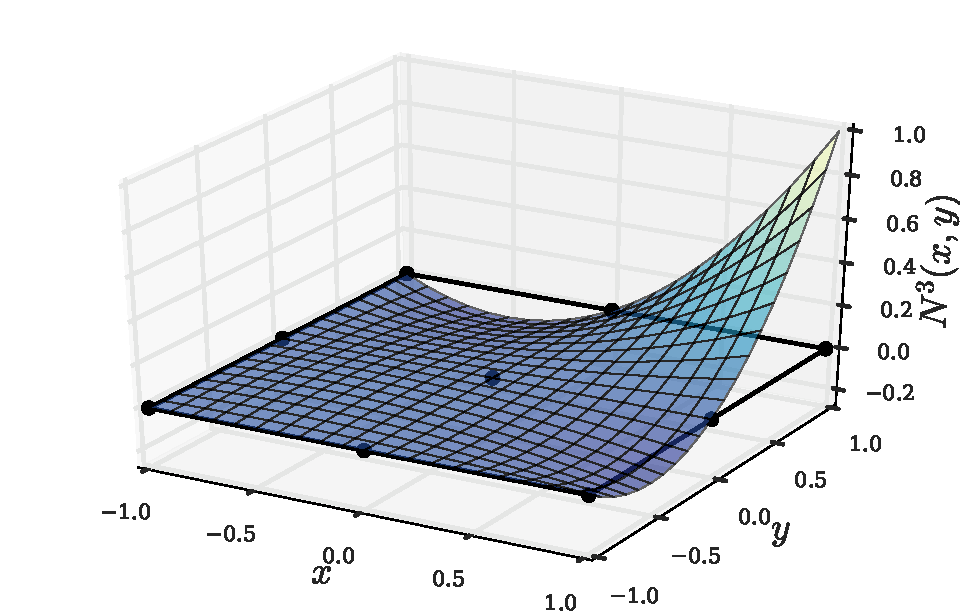
\includegraphics[width=\textwidth]{shape_func-9-nodes-3.pdf}
%		\caption{Shape function $N^3(x,y)$.}
%	\end{subfigure}\,
%%
%	\begin{subfigure}[b]{0.45\textwidth}\qquad
%		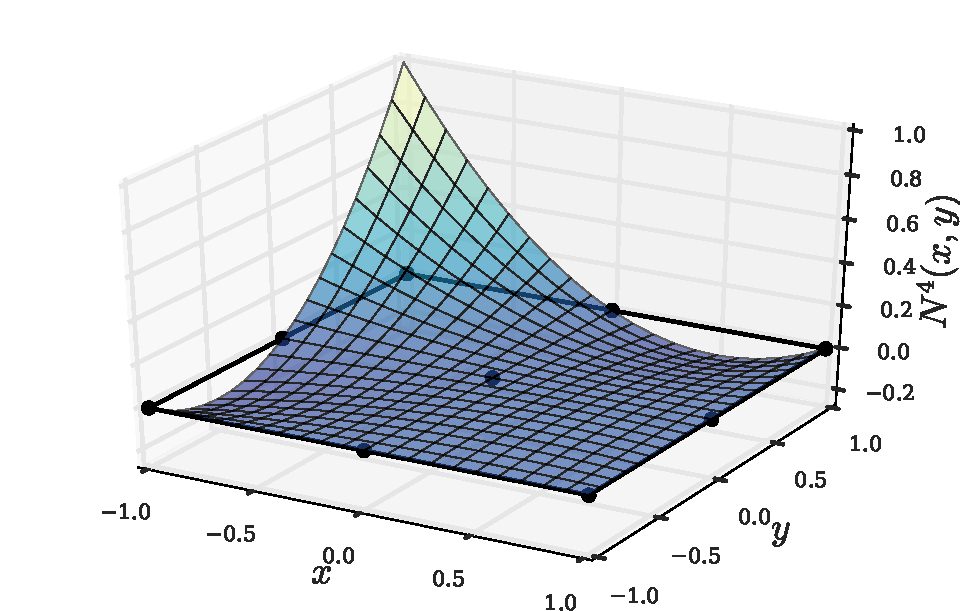
\includegraphics[width=\textwidth]{shape_func-9-nodes-4.pdf}
%		\caption{Shape function $N^4(x,y)$.}
%	\end{subfigure}\\
%	%
%	\begin{subfigure}[b]{0.45\textwidth}\qquad
%		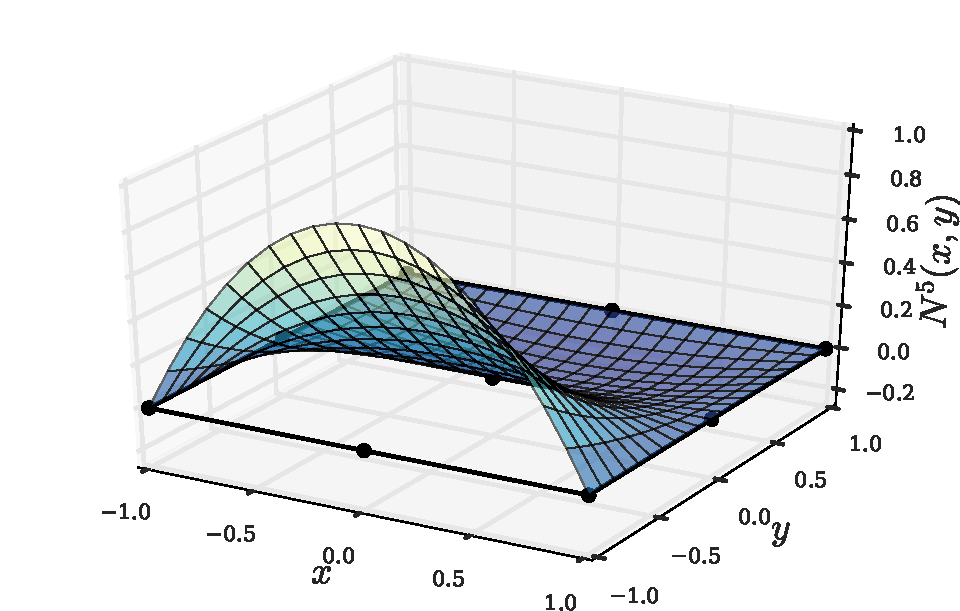
\includegraphics[width=\textwidth]{shape_func-9-nodes-5.pdf}
%		\caption{Shape function $N^5(x,y)$.}
%	\end{subfigure}\,
%%
%	\begin{subfigure}[b]{0.45\textwidth}\qquad
%		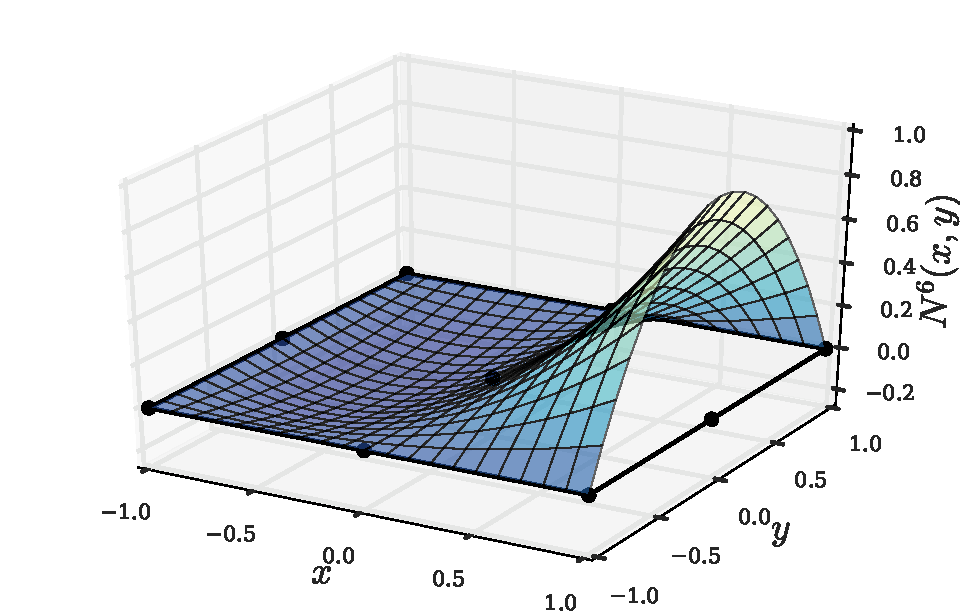
\includegraphics[width=\textwidth]{shape_func-9-nodes-6.pdf}
%		\caption{Shape function $N^6(x,y)$.}
%	\end{subfigure}
%	\caption{Shape functions for a 9-nodes element.}
%	\label{fig:nine-nodes-interp}
%\end{figure}
%%
%\begin{figure} [H]
%	\ContinuedFloat
%	\centering
%	\begin{subfigure}[b]{0.45\textwidth}\qquad
%		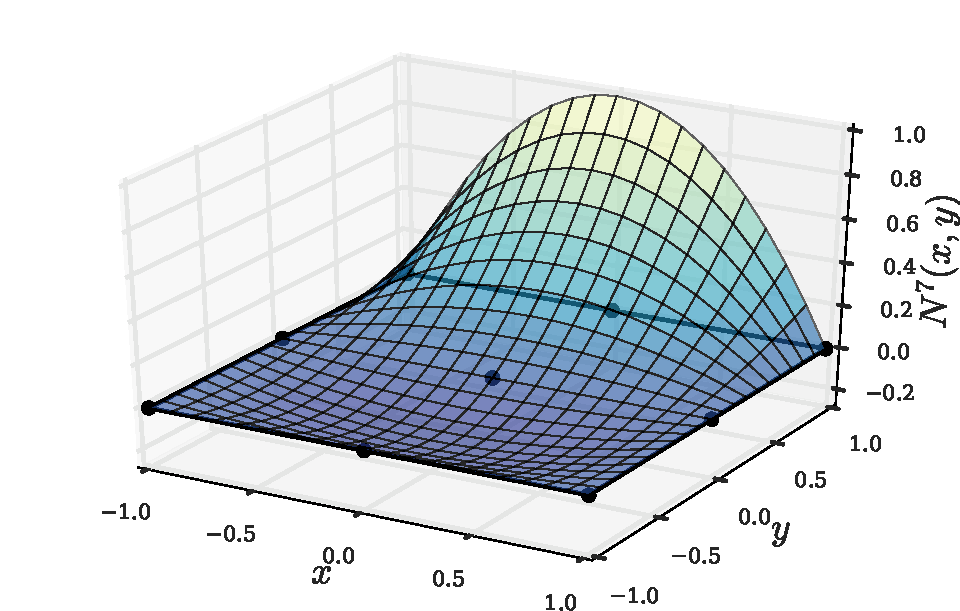
\includegraphics[width=\textwidth]{shape_func-9-nodes-7.pdf}
%		\caption{Shape function $N^7(x,y)$.}
%	\end{subfigure}\,
%%
%	\begin{subfigure}[b]{0.45\textwidth}\qquad
%		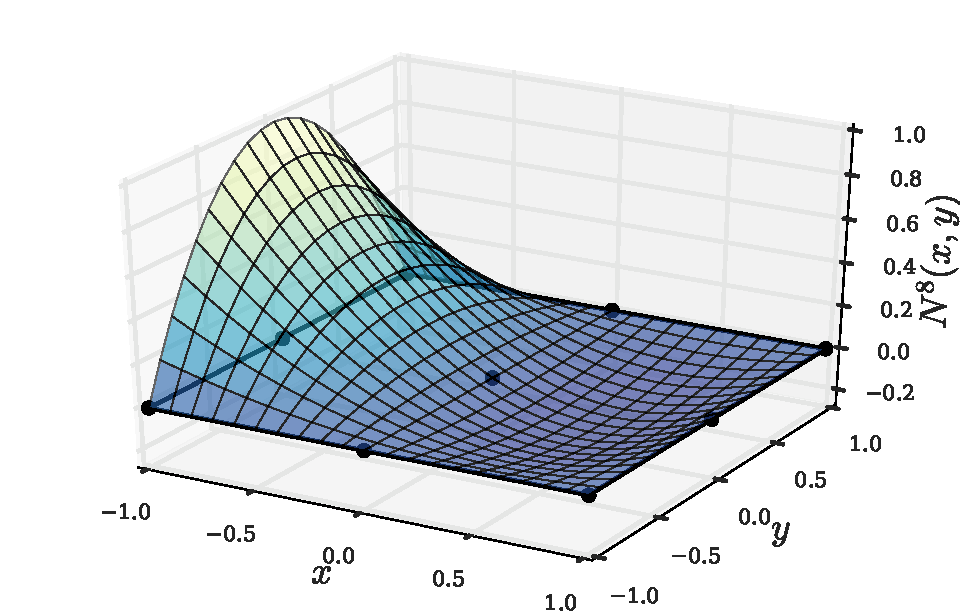
\includegraphics[width=\textwidth]{shape_func-9-nodes-8.pdf}
%		\caption{Shape function $N^8(x,y)$.}
%	\end{subfigure}\\
%	%
%	\begin{subfigure}[b]{0.45\textwidth}\qquad
%		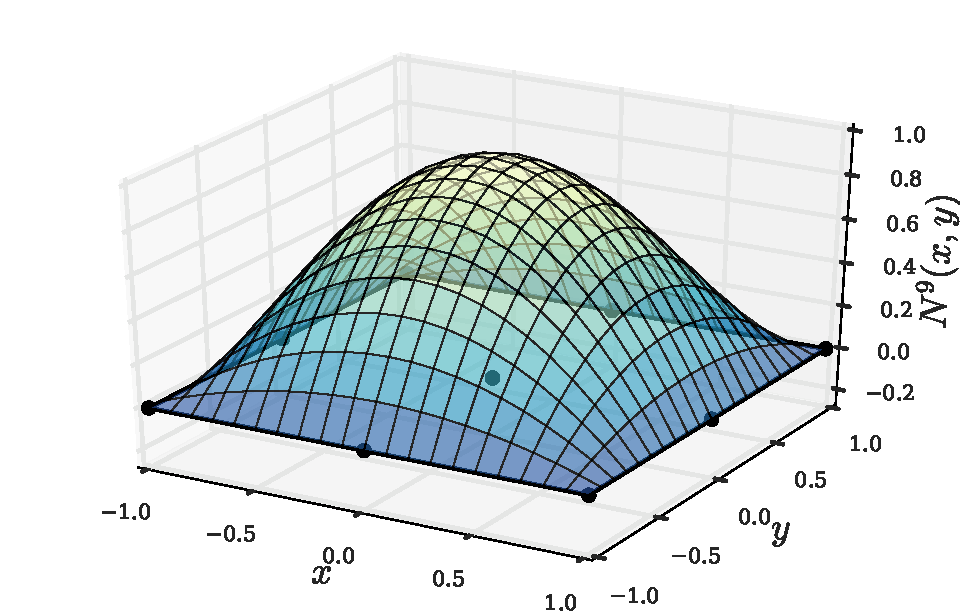
\includegraphics[width=\textwidth]{shape_func-9-nodes-9.pdf}
%		\caption{Shape function $N^9(x,y)$.}
%	\end{subfigure}
%\caption{Shape functions for a 9-nodes element. (Continued)}
%\end{figure}


\begin{tcolorbox}
\paragraph*{Finite element mesh}
Spatial-discretization of the computational domain is in the core of finite element analysis. This corresponds to the partition of the whole domain into {\bf finite elements}. The complete set of finite elements, and its defining attributes, corresponding to a particular domain is termed a {\bf mesh}. If the geometry is irregular the mesh would contain mostly distorted elements with respect to the canonical shape. In the finite element method this is nicely solved using space transformations between the distorted and the canonical shape.

\end{tcolorbox}

%%%%%%%%%%%%%%%%%%%%%%%%%%%%%%%%%%%%%%%%%%%%%%%%%%%%%%%%%%%%%%%%


\section{Interpolation over distorted domains}
So far all the 2D interpolation operations have taken place over perfectly squared domains of side $h$ where the interpolation functions are known at least in terms of the side parameter $h$. In many cases and particularly in finite element methods it is common to find distorted interpolation domains (see \cref{fig:physical}) which difficult the interpolation operation as the interpolation polynomials would be element-dependent and the problem would become impossible to code in a systematic way.


\begin{figure}[h]
\centering
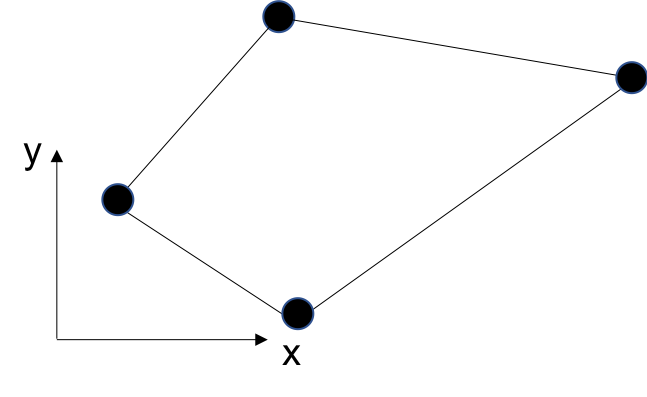
\includegraphics[width=6cm]{rombo}
\caption{Distorted quadrilateral interpolation domain.}
\label{fig:physical}
\end{figure} 

In these cases the solution approach is based upon the continuous mapping of the distorted domain and the functions defined in this space into a constant or canonical element where the interpolation functions are always the same. Moreover, the mapping between both spaces is conducted also using interpolation theory. This idea is explained next with reference to \cref{fig:natural domain}.


\begin{figure}[h]
\centering
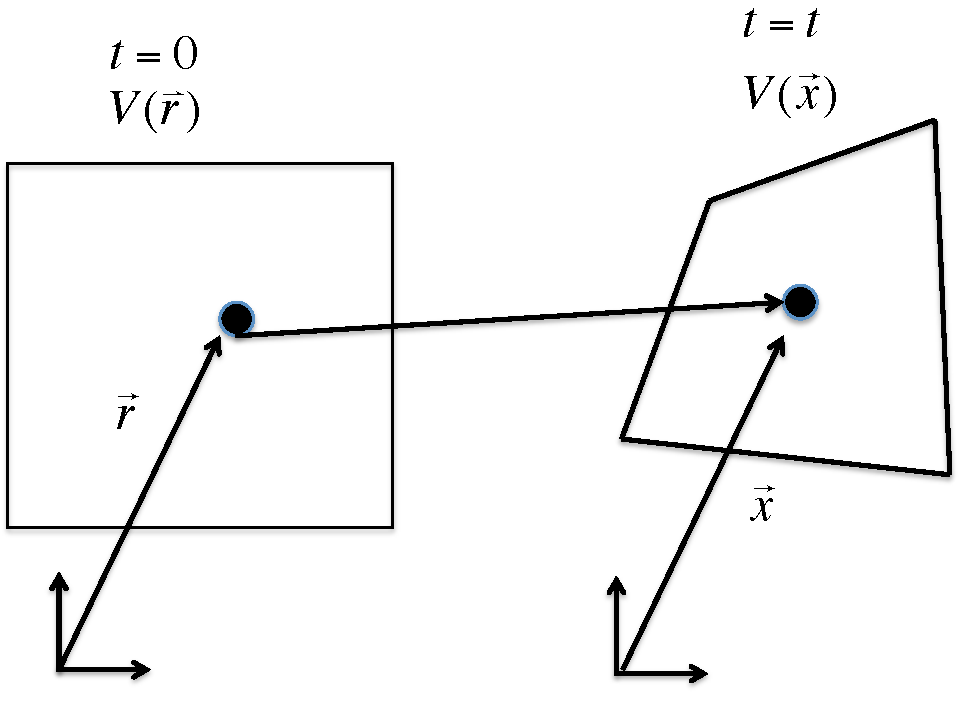
\includegraphics[width=8cm]{figure1.pdf}
\caption{Schematic representation of the one-to-one mapping between points in the physical space (left) and the natural or canonical space (right).}
\label{fig:natural domain}
\end{figure} 

In the figure the space of the distorted domain, and with position vectors $\overrightarrow x$, is termed the physical space as this corresponds to the space of interest in a particular problem. The figure also shows a perfectly squared domain where we denote space coordinates by a position vector $\overrightarrow r$: we refer to this perfectly squared element as the canonical element and to its mathematical space as the natural space. For reasons that will be explained later, it is convenient to  have canonical elements of side $h = 2.0$. Note also that since the canonical element is a constant square of side $h$ the corresponding Lagrange interpolation functions are always the same. This implies that if the interpolation process were to be conducted over the natural space it could be easily coded as it would amount to coding the interpolation functions per se.

In mathematical language the connection between both spaces is written in terms of general functional relations as:

\begin{equation}
\begin{aligned}
x_i &=x_i(\overrightarrow r)\\
r_I &=r_I(\overrightarrow x).
\end{aligned}
\label{eq:trans}
\end{equation}

The first of these functional relationships maps every point $\overrightarrow r$ from the canonical space into a point $\overrightarrow x$ of the physical space. In particular the relationship \ref{eq:trans}(a) can be written using:


\begin{equation}
x_i=N^Q(\overrightarrow r)x^Q.
\label{eq:trans_iso}
\end{equation}


where the physical space has been represented as an interpolated approximation using as the exact functions the coordinates of the nodal points of the physical space. In particular, the first expression provides the position vector $\overrightarrow x$ in the physical space for a point that in the canonical space occupies the position vector $\overrightarrow r$. Similarly, the inverse relation gives the position vector $\overrightarrow r$ in the canonical space for a point that occupies the position vector $\overrightarrow x$ in the physical space. Note that since in \ref{eq:trans}(a) we have used the interpolation functions formulated for the perfectly squared canonical space to approximate the geometry or actual physical space this same transformation can be used to transform functions as explained next.

Assume that $f=f(\overrightarrow x)$ is a function that describes the space variation of a quantity of interest over a given domain.  Using  the mapping \ref{eq:trans} it is also possible to obtain the variation of the quantity in the canonical space after writing:


\[ f=f(\overrightarrow x)\equiv f\lbrack x_i(\overrightarrow r)\rbrack\equiv F(\overrightarrow r). \]

In the above expression $F = F(\overrightarrow r)$ represents the same physical variable but expressed in terms of the position vector in the canonical space. Being able to represent functions in the physical and the canonical space is an important result since it is now possible to conduct interpolation of functions over constant domains as:

\begin{equation}
F(\overrightarrow r)=N^Q(\overrightarrow r)f^Q.
\label{eq:trans_inter}
\end{equation}

Note that as a result of the space transformation \ref{eq:trans}, finding the physical function at a point $r_I$ is equivalent to finding the function at an associated point $x_i$ in the physical domain.


\begin{tcolorbox}

Notebooks 3 and 4 in the REPO make use of Pyhton functions to perform interpolation over two-dimensional domains. In particular, NB4 applies interpolation over arbitrary domains to visualize closed-form solutions.

\end{tcolorbox}

%
\paragraph*{Proposed problems}
\begin{enumerate}

\item \label{punto01} For the computational domain $x\in\lbrack-1.0\;,\;1.0\rbrack$ and 3 nodal points corresponding to $x^1 = -1.0$, $x^2 = +1.0$ and $x^3 = 0.0$ find the Lagrange polynomials $L^1(x)$, $L^2(x)$ and $L^3(x)$.

\item \label{punto02} Verify that the polynomials $L^1(x)$, $L^2(x)$ and $L^3(x)$ satisfy the property $L^I(x^J)=\delta^{IJ}$. 

\item \label{punto03} Implement a Python script that uses the vector of known values of a function $[f^1 , f^2 , f^3 ]$ and the polynomials from problem 1 and compute the interpolating polynomial $p(x)$.

\item \label{punto04} Using $p(x)$ from problem 3 compute and plot the first order derivative of $f(x)$ in the interval $[-1 , 1]$.

\item \label{punto 05} For the function  $f(x) = {x^3} + 4{x^2} - 10$ for $x$ in the range $[-1.0, 1.0]$ find values at nodal points that result from splitting the complete interval into 4 sub-domains each one with 3 nodal points. Using these values implement a local interpolation scheme using 2-nd order local interpolation polynomials. Plot the interpolation polynomial in each sub-domain and the corresponding interpolating function $p(x)$. In the same plot compare $p(x)$ and $f(x)$. Additionally, plot the first derivative of the function obtained from $p(x)$ and $f(x)$.

\item \label{punto 06} For the Runge function defined by:

\[f(x) = \frac{1}{{1 + 25{x^2}}}\]

implement an interpolation scheme using local 1st-order Lagrange polynomials. Use (i) sub-domains of constant size $\Delta x = 0.2$ and (ii) sub-domains whose size decreases towards the edges of the interval.

\item \label{punto 07} Using an independent script (or a notebook) implement a local interpolation scheme using a canonical element of size 2.0 and use it to approximate the Runge function.

\item \label{punto 08} Assume that at the 4 nodal points of a 2D square domain of side $2h$ we know the vector field

\[\overrightarrow u=u(x,y)\widehat i+v(x,y)\widehat j \]

and where $u(x,y)$ and $v(x,y)$ are the scalar rectangular components along the $x$ and $y$ direction of a cartesian coordinate system.

\begin{itemize}
\item[•] Implement an interpolation scheme to compute the vector field $\overrightarrow u\;=\;\overrightarrow u(x,y)$ at an arbitrary point $(x,y)$.
\item[•] Use the interpolation scheme to compute $\varepsilon_{xx}=\frac{\partial u}{\partial x}$ and $\varepsilon_{yy}=\frac{\partial v}{\partial y}$
\item[•] Implement a Python script to visualize the vector field and the scalars $\varepsilon_{xx}$ and $\varepsilon_{yy}$.
\end{itemize}

\item \label{punto 09}
Implement a Python script to visualize analytic (or numerical) solutions available at a set of nodes. Use the following steps;

\begin{itemize}
\item[•] Use external software\footnote{Gmsh is an open source software for pre and post processing of complex 1D, 2D and 3D domains. Meshio is a set of Python scripts to read and write Gmsh readable files using dictionaries.} to define and mesh and arbitrary solution domain.
\item[•] Evaluate the solution at the nodal points of the mesh and store the results into arrays.
\item[•] Use Python triangularization objects together with matplotlib routines to visualize the solution.
\end{itemize}


\end{enumerate}
